\section{The Graphic User Interface}

When launching the GUI, the home screen appears like this :\\


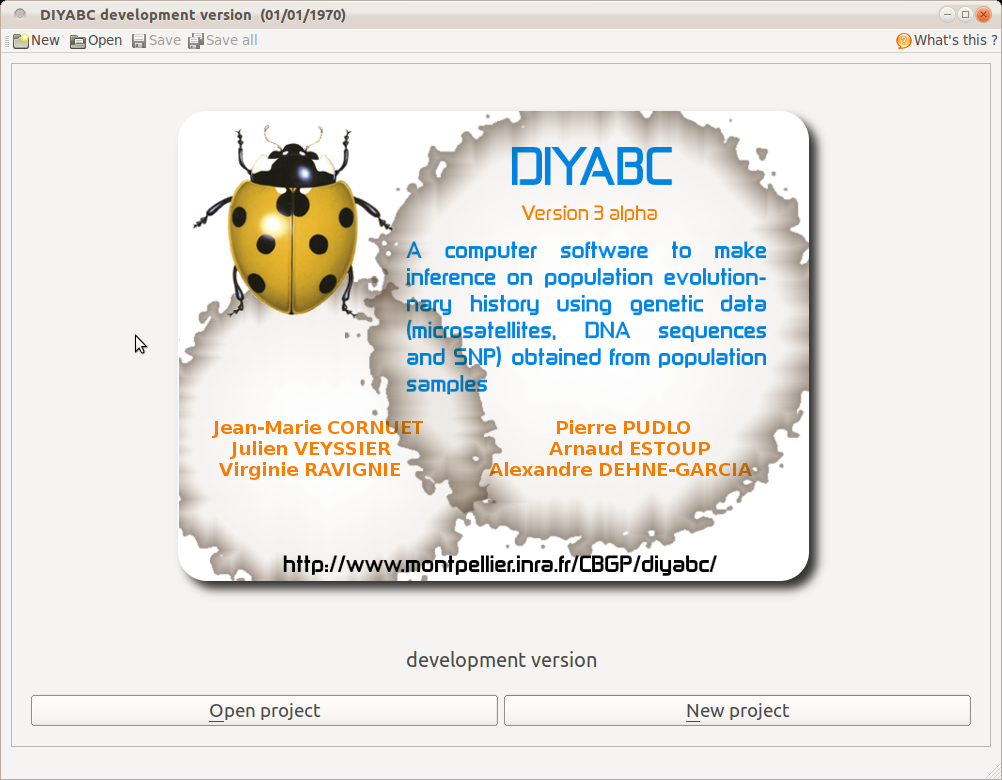
\includegraphics[scale=0.4]{gui_pictures/Capture-DIYABC-1.png} 

You can already notice that $DIYABC$ works with projects. This notion is new to version 2 of $DIYABC$. It is explained in subsection 3.1.

\subsection{What is a $DIYABC$ Project ?}

\label{doc_openProjectButton}
A $ DIYABC $ project is a unit of work materialized by a specific and unique directory. A project is defined by at least one observed data set and one reference table header file. These files are located in the \emph{Project directory} which name includes an identifier, the date of creation and a number (between 1 and 100).\\

The header file, always named \texttt{header.txt}, contains all information necessary to compute a reference table associated with the data : i.e. the scenarios, the scenario parameter priors, the characteristics of loci, the loci parameter priors and the summary statistics to compute.
As soon as the first records of the reference table have been saved in the reference table file,  always named \texttt{reftable.bin} and also included in the project directory, the project is "locked". This means that the header file can not be changed anymore. If one needs to change a scenario or a parameter prior, or a summary statistics, a new project needs to be defined. This is to guarantee that all subsequent actions performed on the project are in coherence with the current data and header files. It is of course strongly advised NOT to move files among projects.
Incidentally, the \texttt{header.txt} file is only built when the project has been saved, the information progressively input by the user being saved in a series of temporary files.\\

Once a sufficiently large reference table has been simulated, analyses can be performed. Their different output files are copied to the \emph{analysis} directory included in the project directory, and containing as many directories as analyses performed. Hence, it is now much easier to know with certainty the conditions of each analysis.    

\subsection{Options of the home screen}
\label{doc_newSNPProjectButton}
The home screen above has two menus and several buttons.\\ 
Let's start with the menus. Below are shown all submenus :

\begin{center} 
\begin{tabular}{cc}
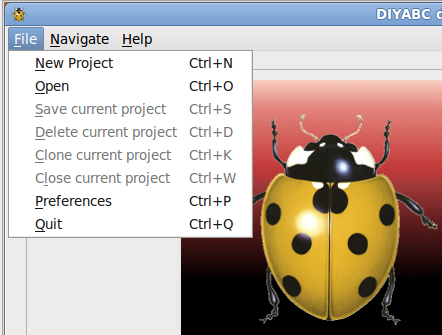
\includegraphics[scale=0.5]{gui_pictures/Capture-DIYABC-2.png} & 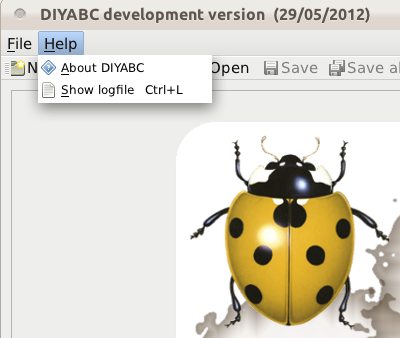
\includegraphics[scale=0.5]{gui_pictures/Capture-DIYABC-3.png}\\
\end{tabular}
\end{center}

The \texttt{File} menu has seven options, namely \texttt{New project}, \texttt{Open project}, \texttt{Open recent projects}, \texttt{Save all projects}, \texttt{Settings}, \texttt{Simulate data set(s)} and \texttt{Quit}. All are self explanatory.\\
The \texttt{Help} menu has two options : \texttt{About DIYABC} which opens up a small window providing the names and address of the authors and \texttt{Show logfile} which gives access to a logfile viewer in which are recorded all actions and messages about the execution of the GUI.\\ 
Just below the menu are five shortcuts to main \texttt{File} menu options.\\

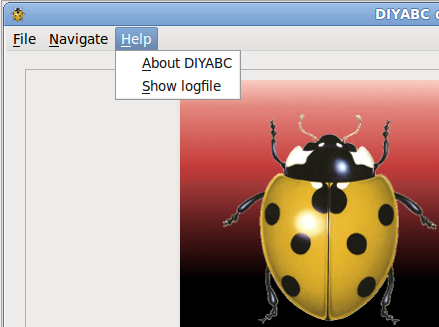
\includegraphics[scale=0.4]{gui_pictures/Capture-DIYABC-4.png}\\
 
On the right, the field \texttt{What's this ?} is an another way to get help on a specific GUI object :\\
 
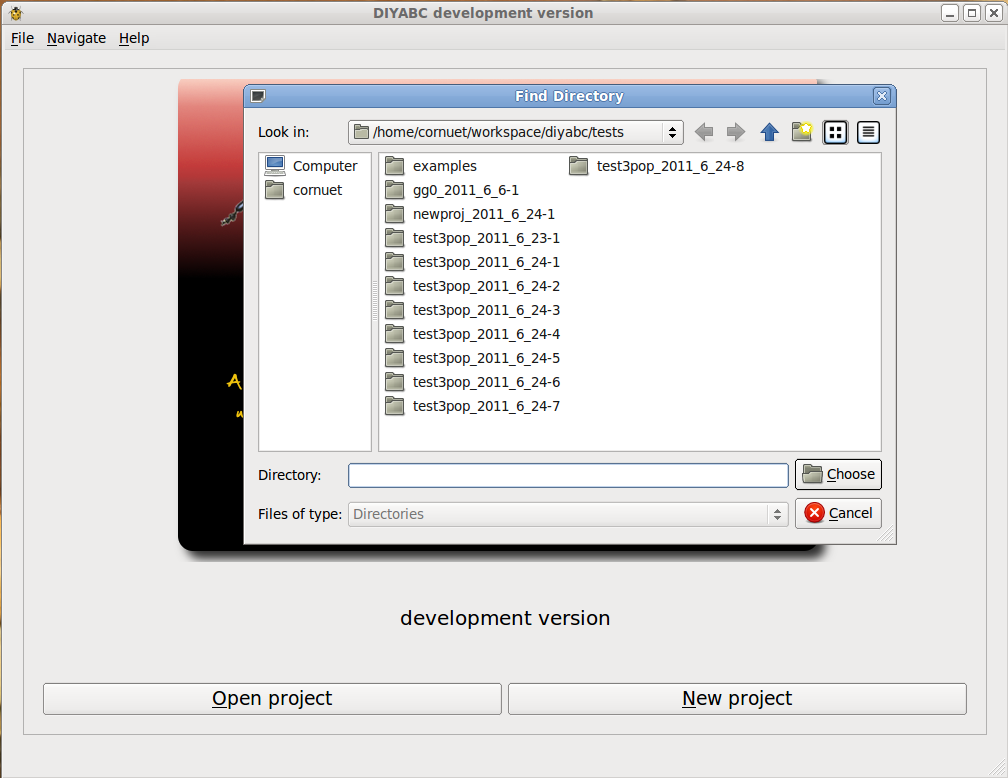
\includegraphics[scale=0.4]{gui_pictures/Capture-DIYABC-5.png}\\ 

Eventually, below the logo, there are three buttons which are duplicate shortcuts :\\
 
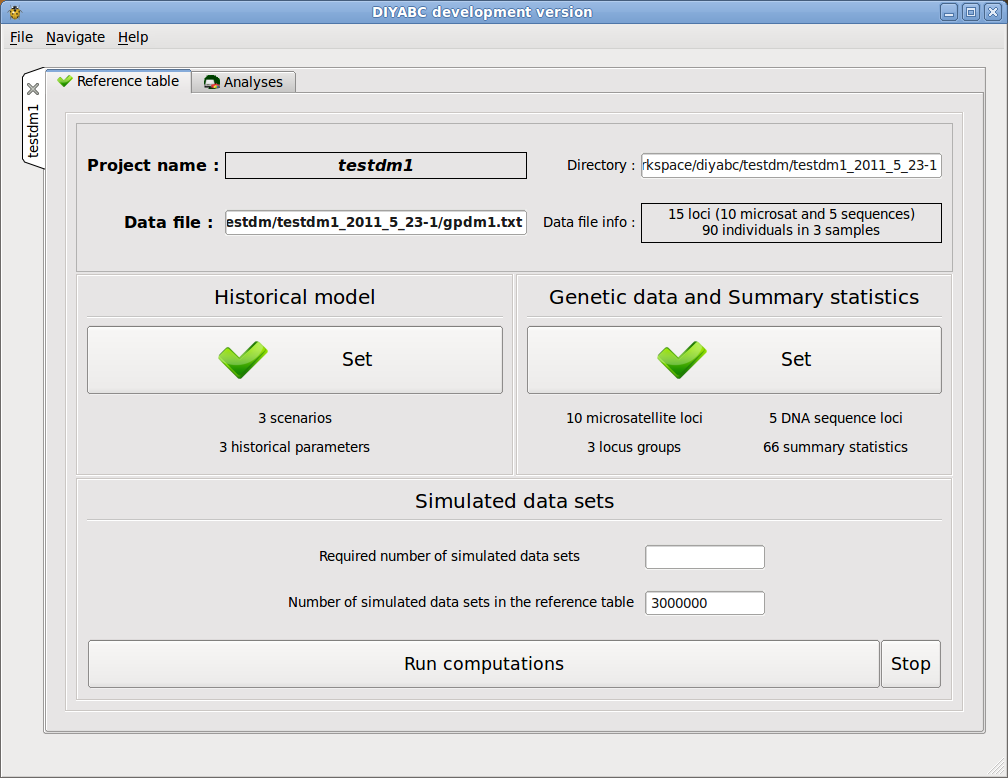
\includegraphics[scale=0.4]{gui_pictures/Capture-DIYABC-6.png}\\ 


  
%Clicking on the \fbox{\textsf{Open project}} button opens up the following frame:\\

%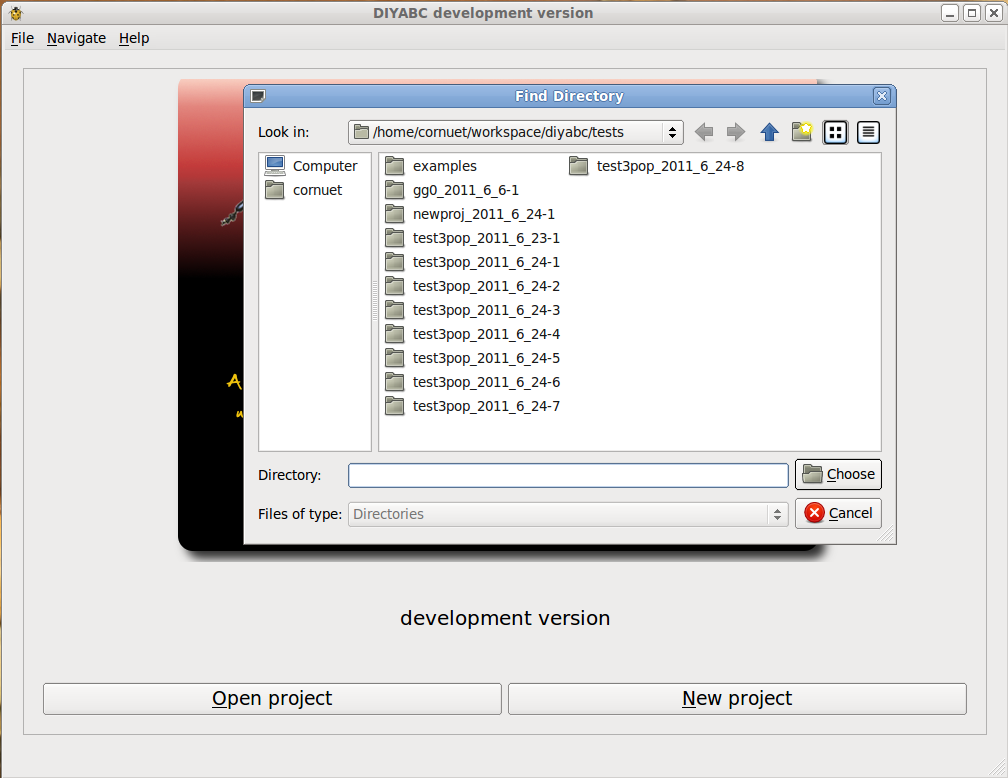
\includegraphics[scale=0.4]{gui_pictures/Capture-DIYABC-5.png} 

%To select a project, you just double click on the corresponding directory.
%\newpage
% The following screen then appears :\\

%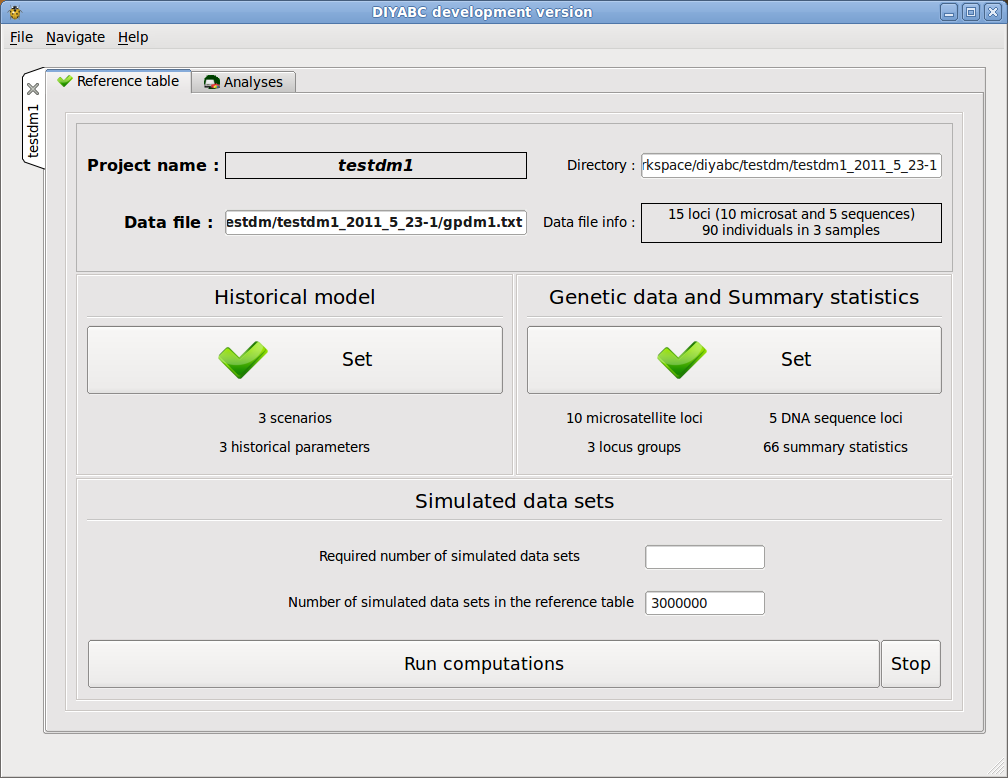
\includegraphics[scale=0.35]{gui_pictures/Capture-DIYABC-6.png} 

%We will go back later to the description of this screen.
%\begin{itemize}
% \item 
%  Cliking on the \fbox{\textsf{New project}} opens up the screen below requiring a name for the new project :\\
%\begin{center}
%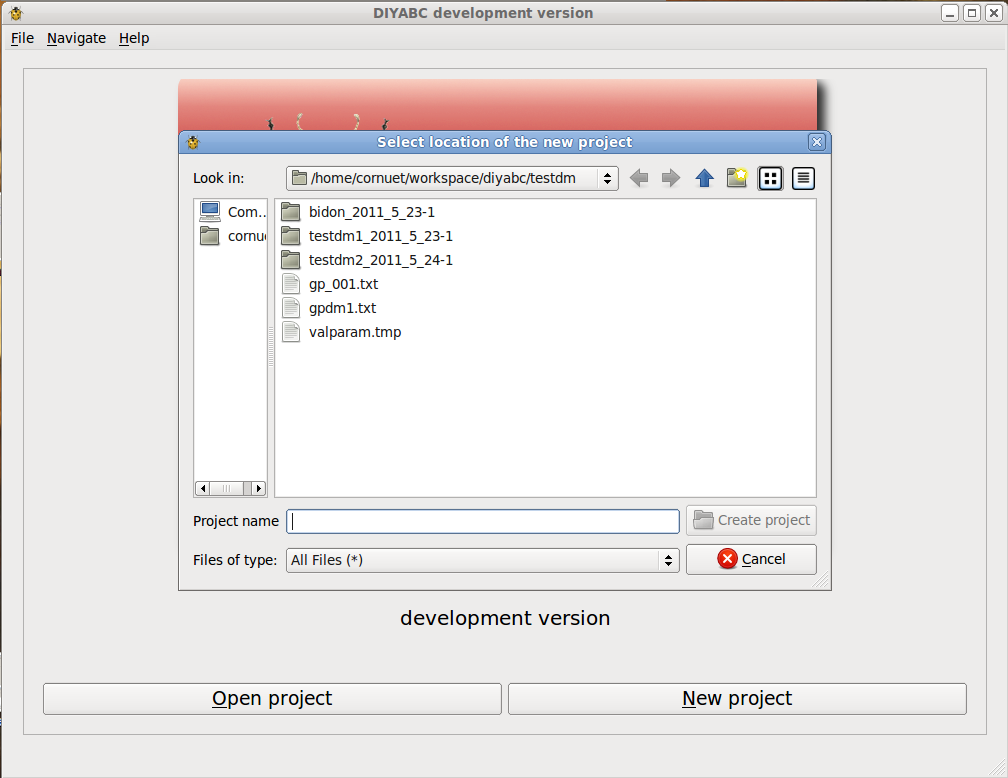
\includegraphics[scale=0.35]{gui_pictures/Capture-DIYABC-7.png} 
%\end{center}
%\item
%After giving a name to new project and cliking on \fbox{\textsf{OK}}, the following screen appears :\\ 

%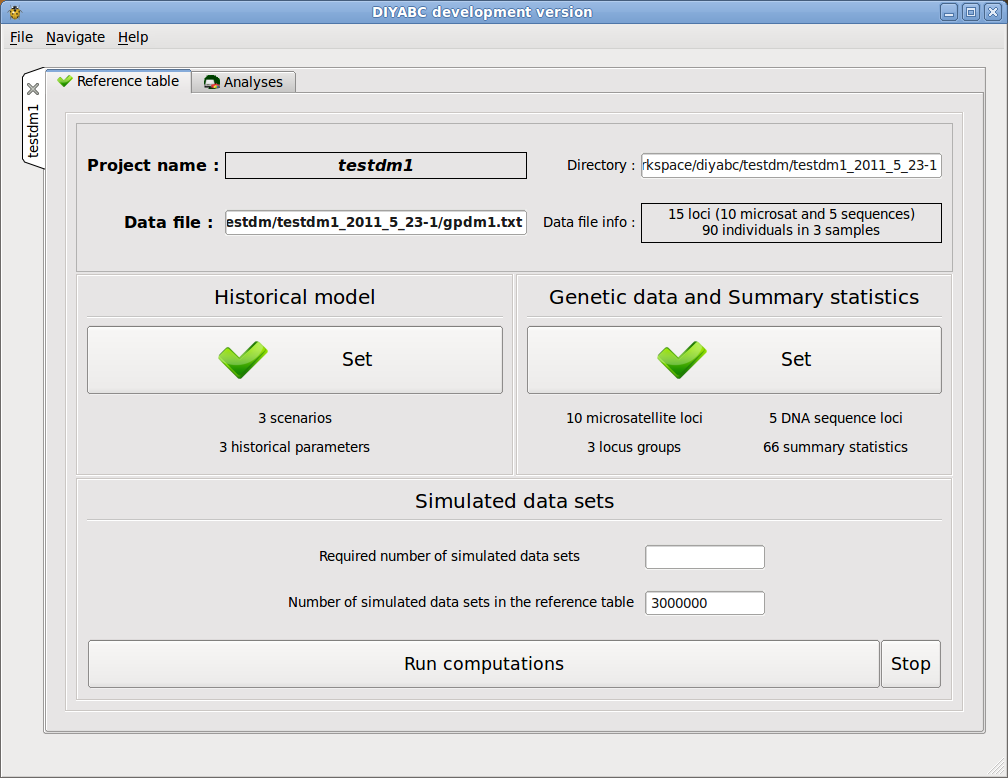
\includegraphics[scale=0.35]{gui_pictures/Capture-DIYABC-6.png} 

%\end{itemize}

\subsection{Defining a new project}
Defining a new project requires different steps which are not the same whether the data are SNPs or microsatellites/DNA sequences (MSS). 
Let start with an MSS project : click on one of the following :
\begin{itemize}
 \item \texttt{File} menu $>$ \texttt{New project} $>$ \texttt{Microsatellites and/or sequences}
 \item the menu shortcut \texttt{New MSS}
 \item the bottom left button \fbox{\textsf{New Microsat/Sequence project}}
\end{itemize}
or press simultaneously the \texttt{Control} and \texttt{M} keys.\\
A new window appears in which the user can choose a location and a name for the new project as shown below :\\

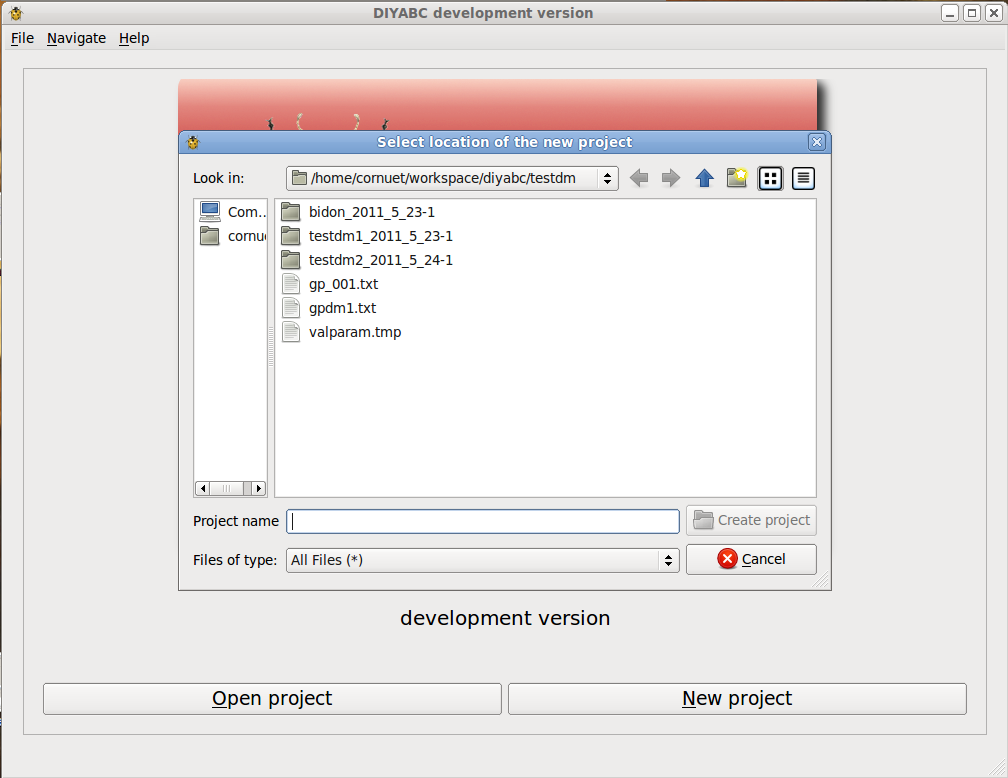
\includegraphics[scale=0.35]{gui_pictures/Capture-DIYABC-7.png} 

Let's enter \textbf{demo1} as the project name and click on the \fbox{\textsf{Create project}} button.\\
The following screen appears :\\

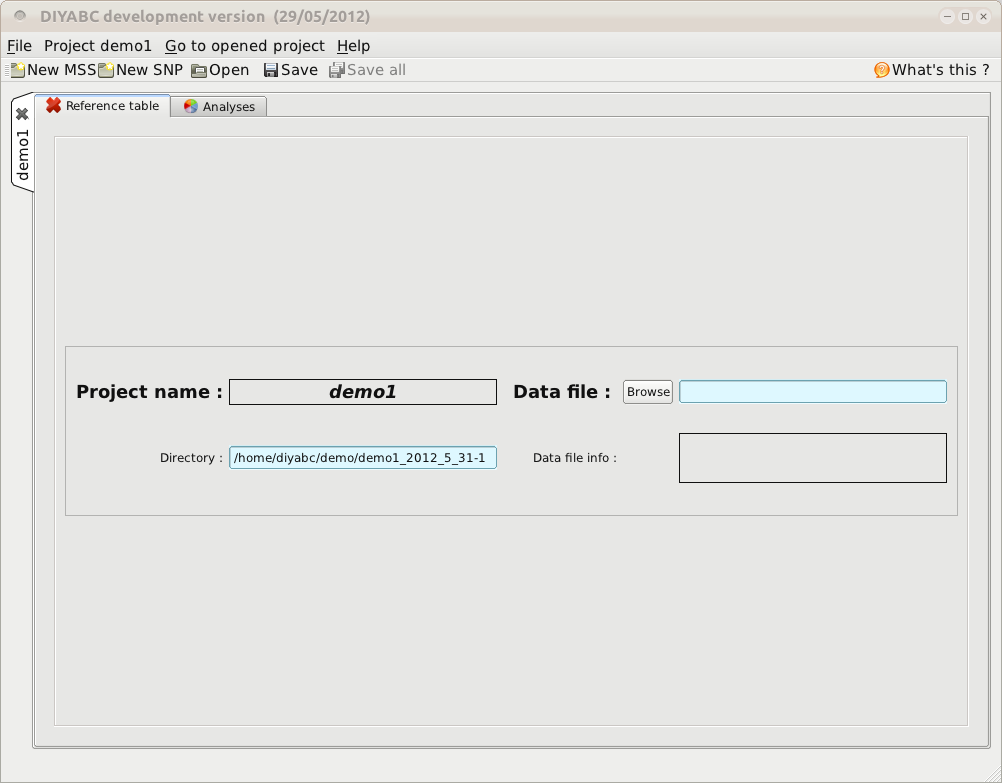
\includegraphics[scale=0.35]{gui_pictures/Capture-DIYABC-8.png} 

The \textbf{demo1} project and all its future files will be located in the directory \texttt{demo1\_2012\_5\_31-1}.

\subsubsection{Step 1 : choosing the data file}
We next need to choose the data file of the project. This is performed by clicking on the corresponding \fbox{\textsf{Browse}} button (previous screen).  The usual file browsing screen appears (below) and one has to select a Genepop format data file, here \texttt{data1.mss}. \\

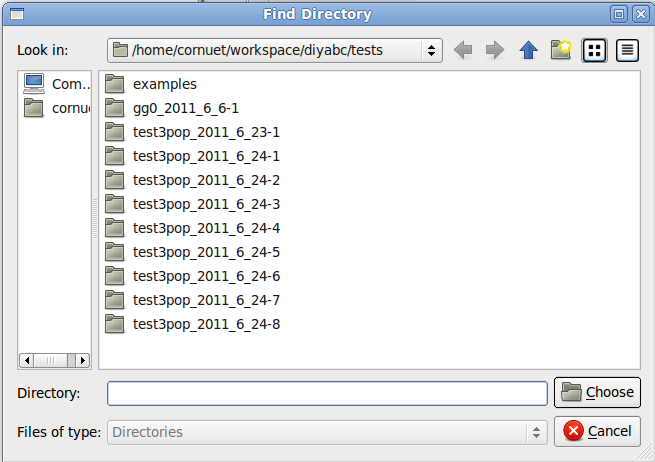
\includegraphics[scale=0.35]{gui_pictures/Capture-DIYABC-9.png} 
\\
Clicking on the \fbox{\textsf{Open}} button leads  to the following screen with the edit field filled with the name of the data file and some characteristics of this data file appearing on the screen (number of loci, individuals and samples).\\
Below these fields are two panels indicating that we need to provide information about the Historical model (left panel) and about the Genetic data and associated Summary statistics (right panel). The red crosses on both panels will change to green checks once the corresponding information will be completed.\\ 
\\
\\
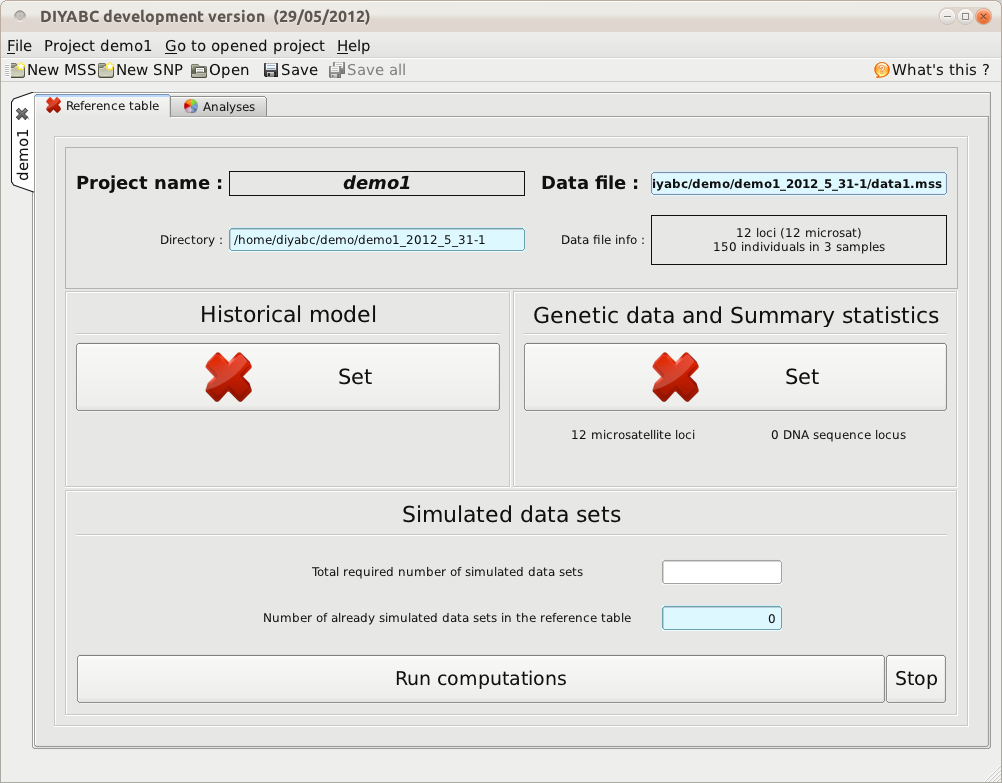
\includegraphics[scale=0.35]{gui_pictures/Capture-DIYABC-10.png} 
\newpage
\subsubsection{Inform the Historical model}
Click on the corresponding \fbox{\textsf{Set}} button. The following screen, familiar to users of previous versions, appears:\\

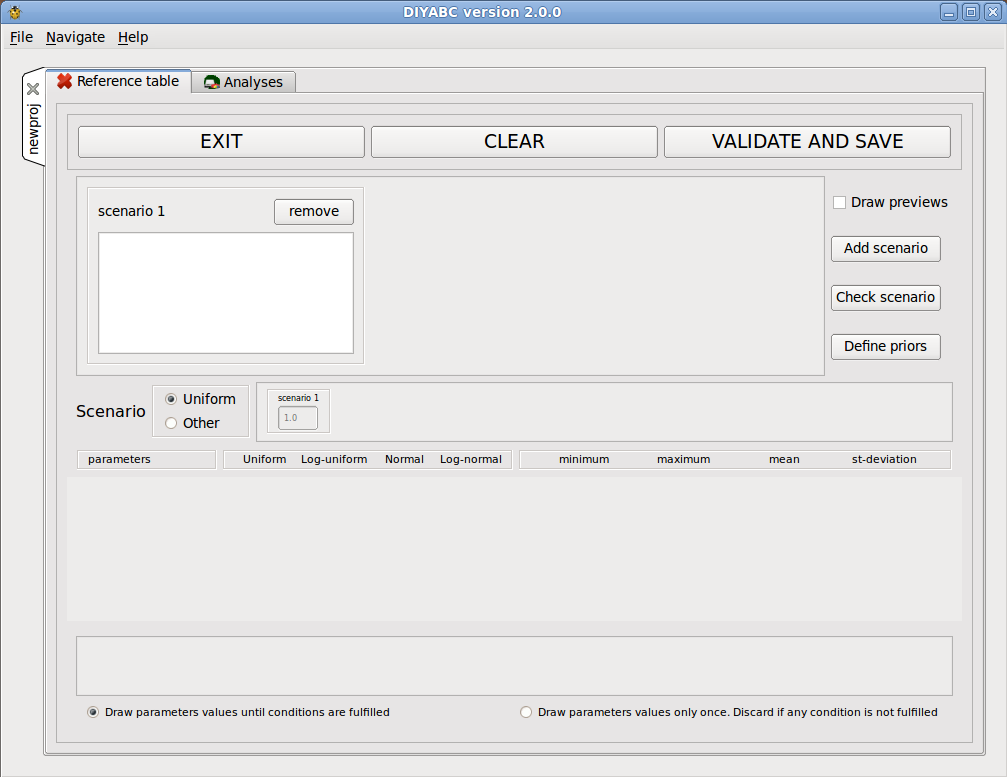
\includegraphics[scale=0.35]{gui_pictures/Capture-DIYABC-11.png} 

Let's enter a simple scenario in scenario 1 edit window and click on the \fbox{\textsf{Define priors}} button. We get this :\\

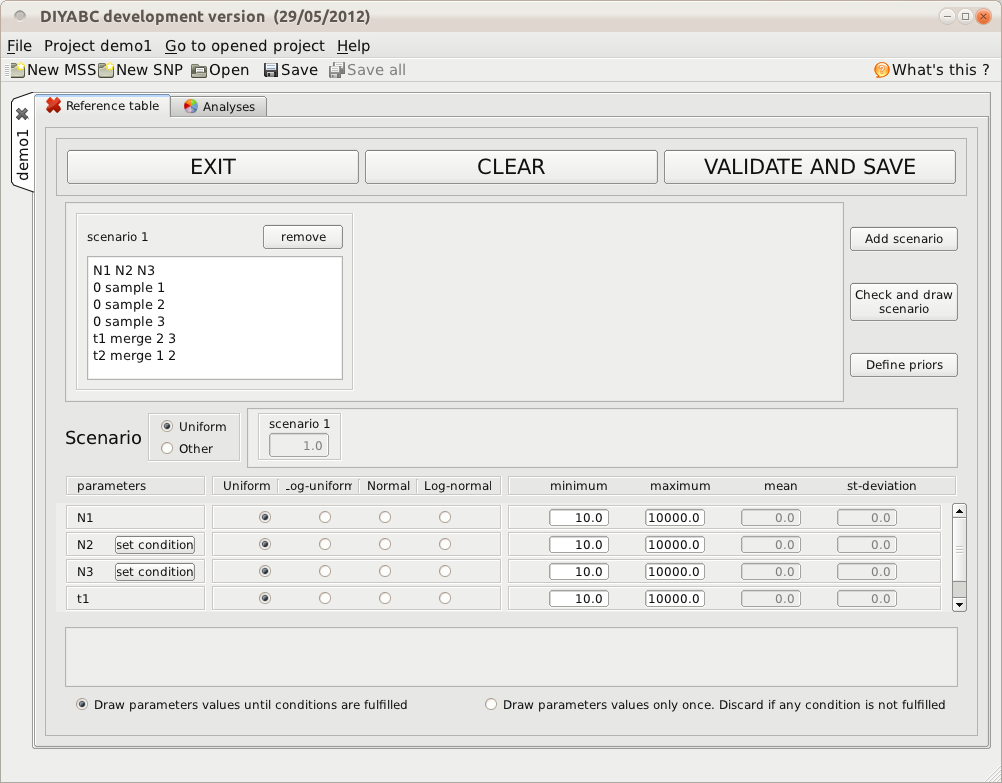
\includegraphics[scale=0.35]{gui_pictures/Capture-DIYABC-12.png} 

The parameter prior frame allows to choose the prior density of each parameter. A parameter is anything in the scenario that is not a keyword (here \texttt{sample} and \texttt{merge}), nor a numeric value. In our example scenario, parameters are hence : \texttt{N1, N2, N3, t1} and \texttt{t2}. In our example, we need to set the priors on \texttt{t1} and \texttt{t2} such that \texttt{t2}$>$  \texttt{t1}. We can do it either by using the \texttt{set condition} button or by playing with the minimum and maximum values of the two parameters.\\

If we click on the \fbox{\textsf{Check scenario}} button, the logic of the scenario is checked and if it is found OK, and if the scenario is drawable, the drawing appears on a new frame : \\

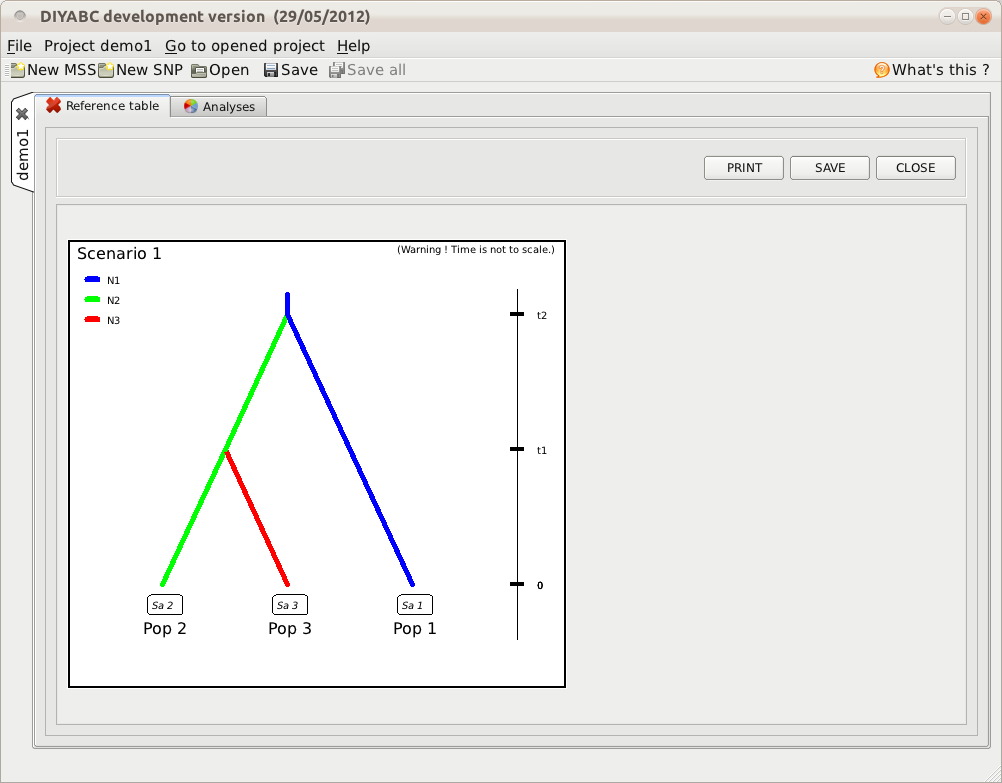
\includegraphics[scale=0.35]{gui_pictures/Capture-DIYABC-13.png} 

The scenario can be saved by clicking on the \fbox{\textsf{SAVE}} button. The frame can be close by clicking on the \fbox{\textsf{CLOSE}} button.\\

Since the scenario has been checked, we can validate and save the historical model by clicking on the  \fbox{\textsf{VALIDATE AND SAVE}} button (bottom screen of p 21). We then go back to the project screen in which the historical model has now received the green check sign.\\

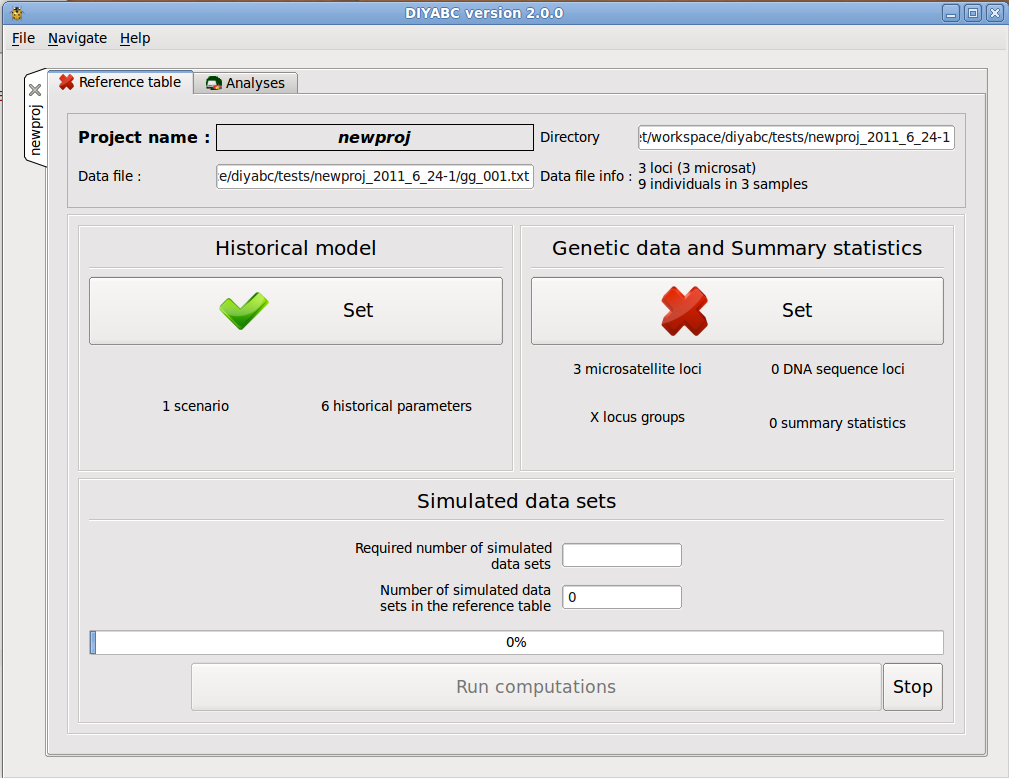
\includegraphics[scale=0.35]{gui_pictures/Capture-DIYABC-14.png} 

 \newpage
\subsubsection{Inform the Genetic model}

Click on the corresponding \fbox{\textsf{Set}} button. We get the following screen : \\

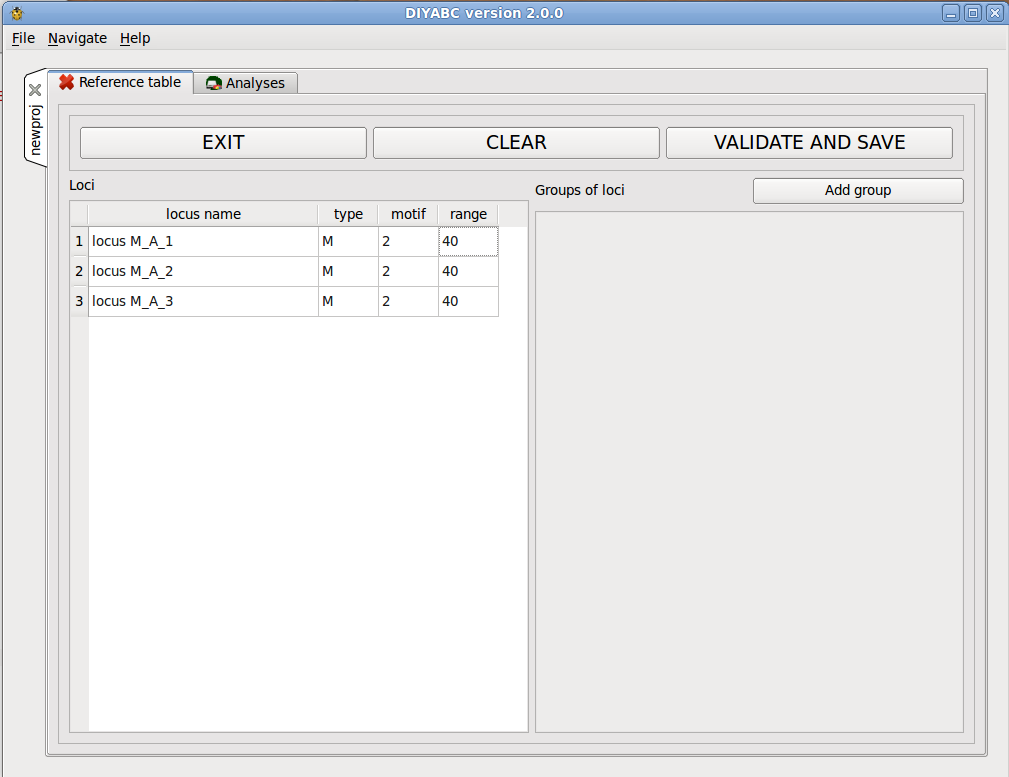
\includegraphics[scale=0.35]{gui_pictures/Capture-DIYABC-15.png} 

On the left part of the screen, there is the list of loci, with their type (M for microsatellites or S for DNA sequences) and the motif size and range for microsatellite loci only. Actually, the values for motif size and range are just default values and do not necessarily correspond to the actual data. The user who knows the real values for its data is required to set the correct values at this stage. If the range is too short to include all observed values, a message appears in a box asking to enlarge the corresponding range. Note that the range is measured in number of motifs, so that a range of 40 for a motif length of 2 bp means that the difference between the smallest and the longest alleles should not exceed 80 bp. It is worth stressing that the indicated allelic range (expressed in number of continuous allelic states) corresponds to a potential range which is usually larger than the range observed from the analyzed dataset (cf. all possible allelic states have usually not been sampled). In practice it is difficult to assess the actual microsatellite constraints on the allelic range; to do that one need allelic data from several distantly related populations/sub-species as well as related species which is rarely the case (\citep[see][]{PDD1998}; \citep{E2002}). We achieved a meta-analysis from numerous primer notes documenting the microsatellite allelic ranges of many (i.e. > 100) different species (and related species). We used the corrective statistical treatment on such data proposed by \citep{PDD1998}. Our results pointed to a mean microsatellite allelic range of 40 continuous states (hence the default allelic range value of 40 mentioned in the program). We also found, however, that range values greatly varied among species and among loci within species (unpublished results). We therefore recommend to use the following pragmatic behaviour when considering the allelic range of your analysed microsatellite dataset: (i) if the difference in number of motif of your locus is < 40 motifs in the analysed dataset then leave the default allelic range value of 40. (ii) if the difference in number of motif of your locus is > 40 motifs in your dataset then take Max\_allele\_size – Min\_allele\_size)/motif size + say 10 additional motifs to re-define the allelic range of the locus in the corresponding DIYABC panel (e.g. (200 nu – 100 nu)/2 + 10 = 50+10 = 60 as allelic range).\\
We then need to define at least one group of loci by clicking on the \fbox{\textsf{Add group}} button. We get this :\\

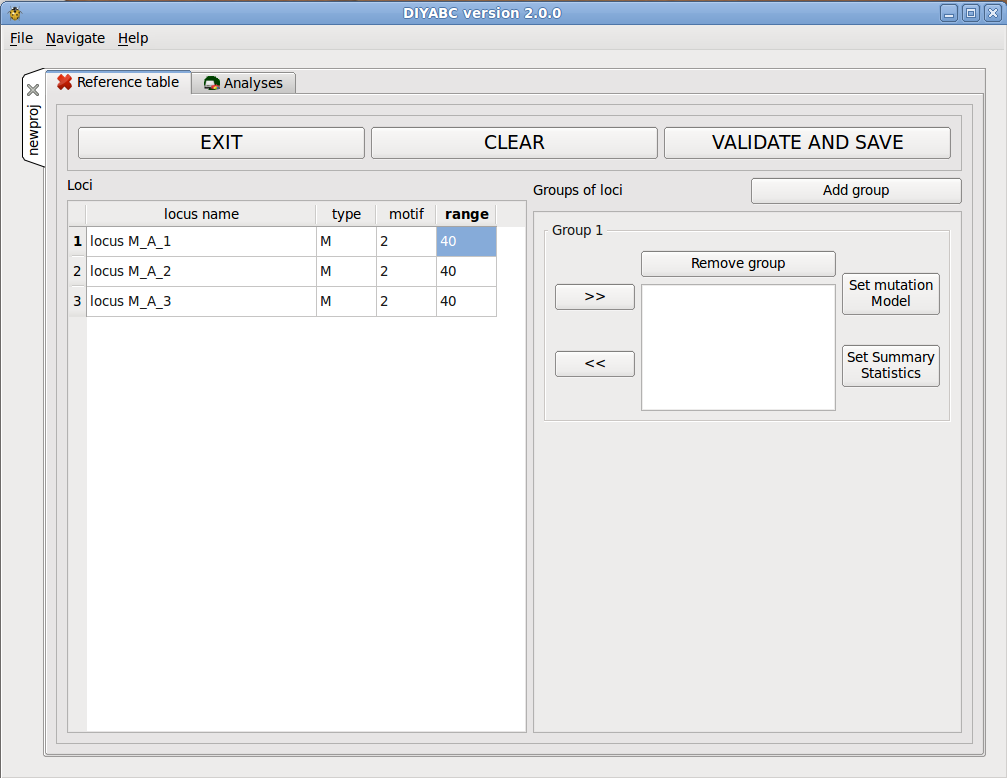
\includegraphics[scale=0.35]{gui_pictures/Capture-DIYABC-16.png} 

Suppose we want all loci in the same group because we consider that they all have similar mutational modalities. We select them like in any table, extending the selection with the \texttt{Shift} and \texttt{Control} keys (see below) : \\

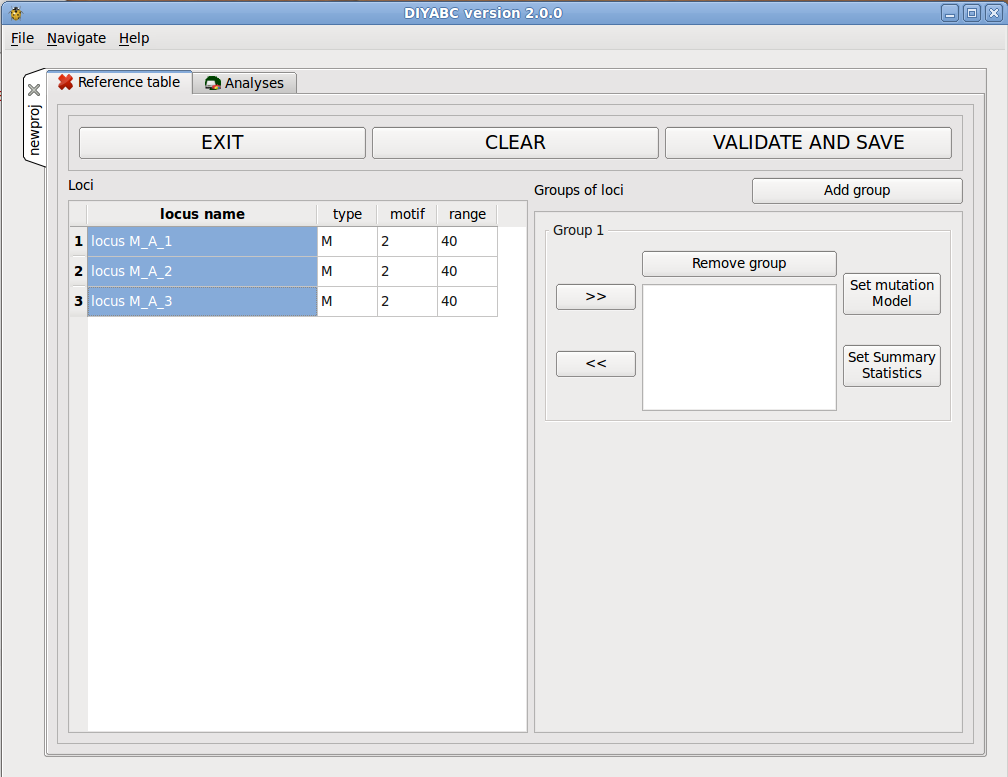
\includegraphics[scale=0.35]{gui_pictures/Capture-DIYABC-17.png} 

and then pressing the \fbox{\textsf{$ >> $}} button : \\

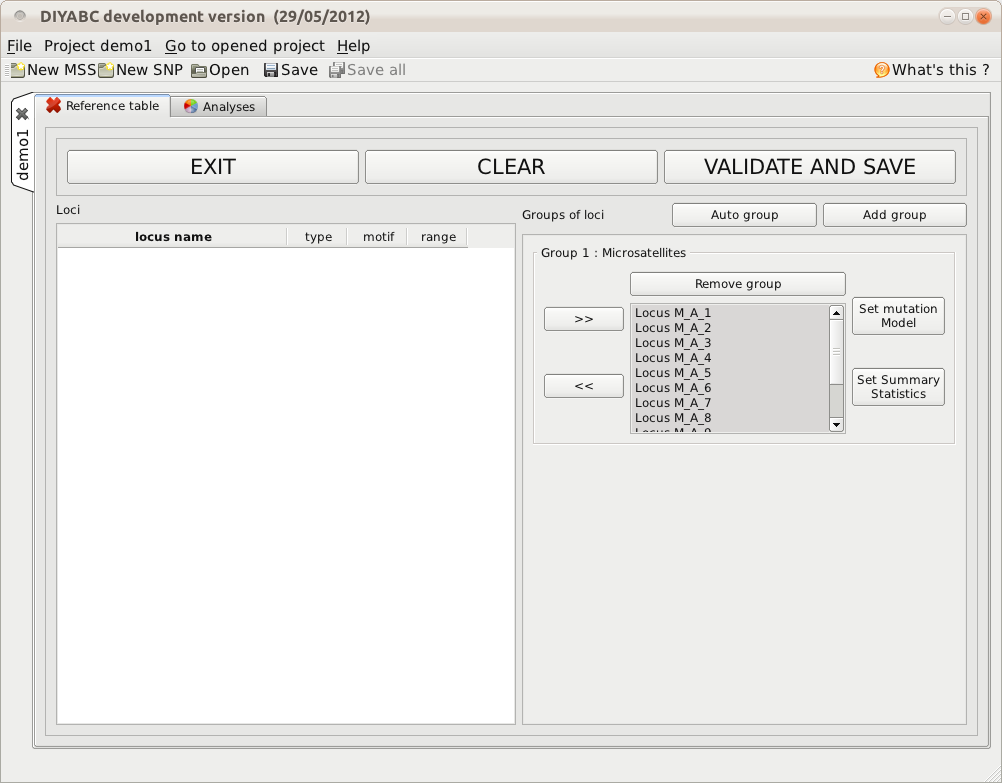
\includegraphics[scale=0.35]{gui_pictures/Capture-DIYABC-18.png}

Note that the \fbox{\textsf{Auto group}} button would have produced the same result of putting all the microsatellite loci in the same group.\\  

We then need to define the mutation model and the summary statistics of the locus group. Clicking on the \fbox{\textsf{Set mutation model}} button, the following screen appears :\\

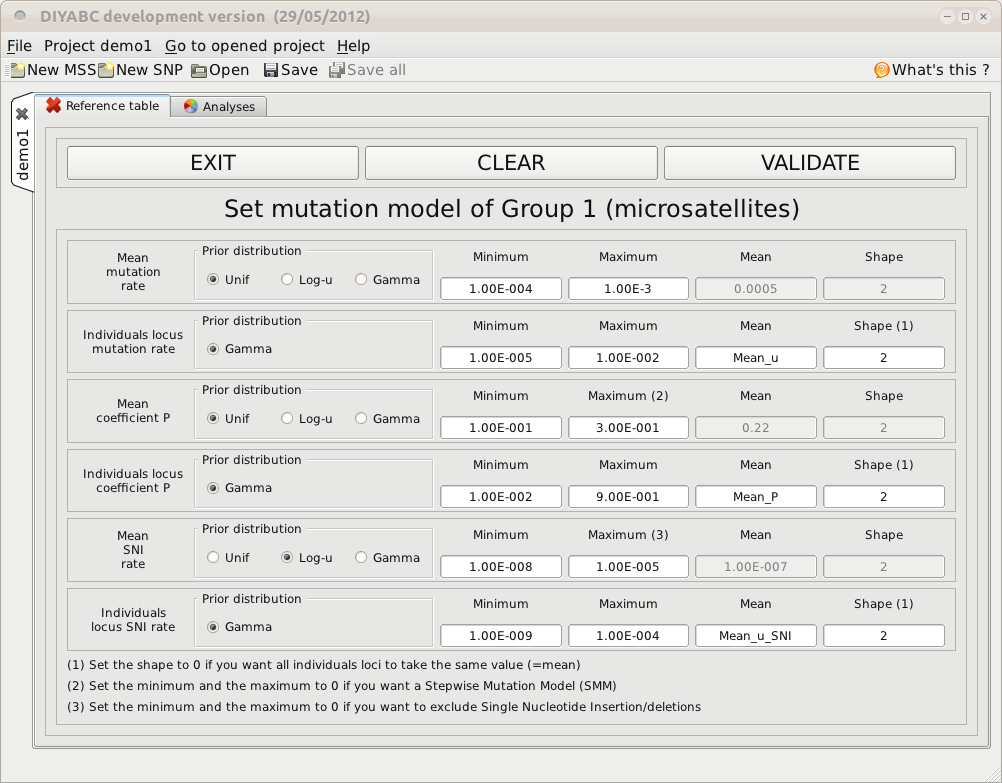
\includegraphics[scale=0.35]{gui_pictures/Capture-DIYABC-19.png} 

Once the mutation model of Group 1 is defined, we click on the \fbox{\textsf{VALIDATE}} button to go back to the previous screen. Clicking on the \fbox{\textsf{Set Summary statistics}} button, we get the following screen :\\ 

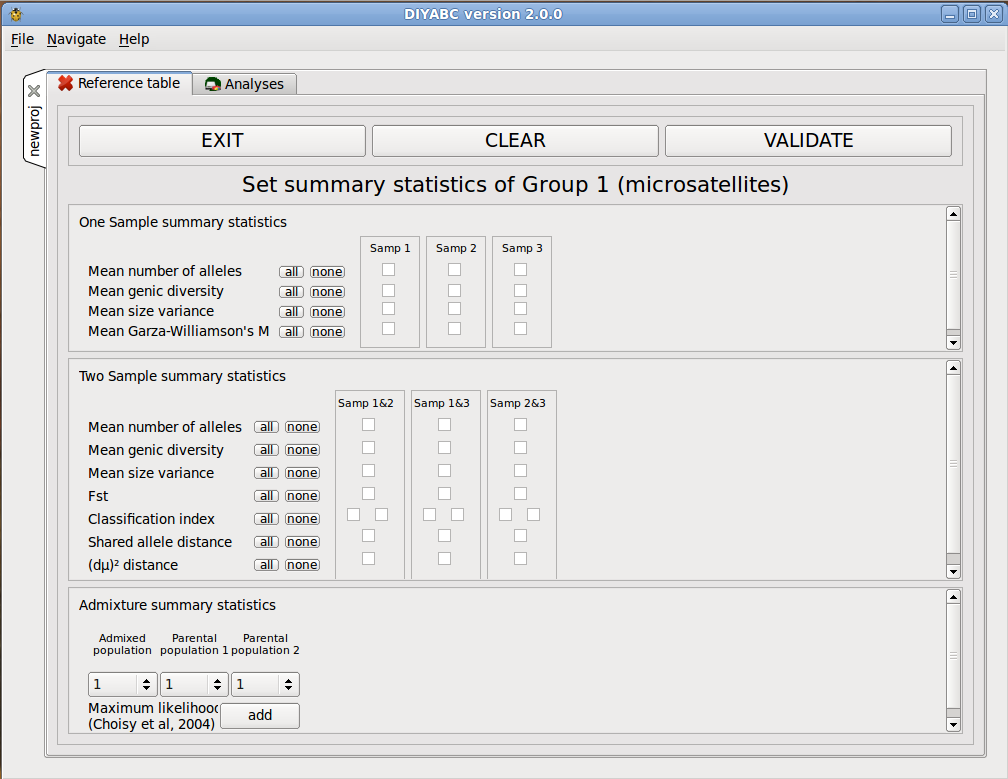
\includegraphics[scale=0.35]{gui_pictures/Capture-DIYABC-20.png} 

We define summary statistics by checking the corresponding boxes :\\ 

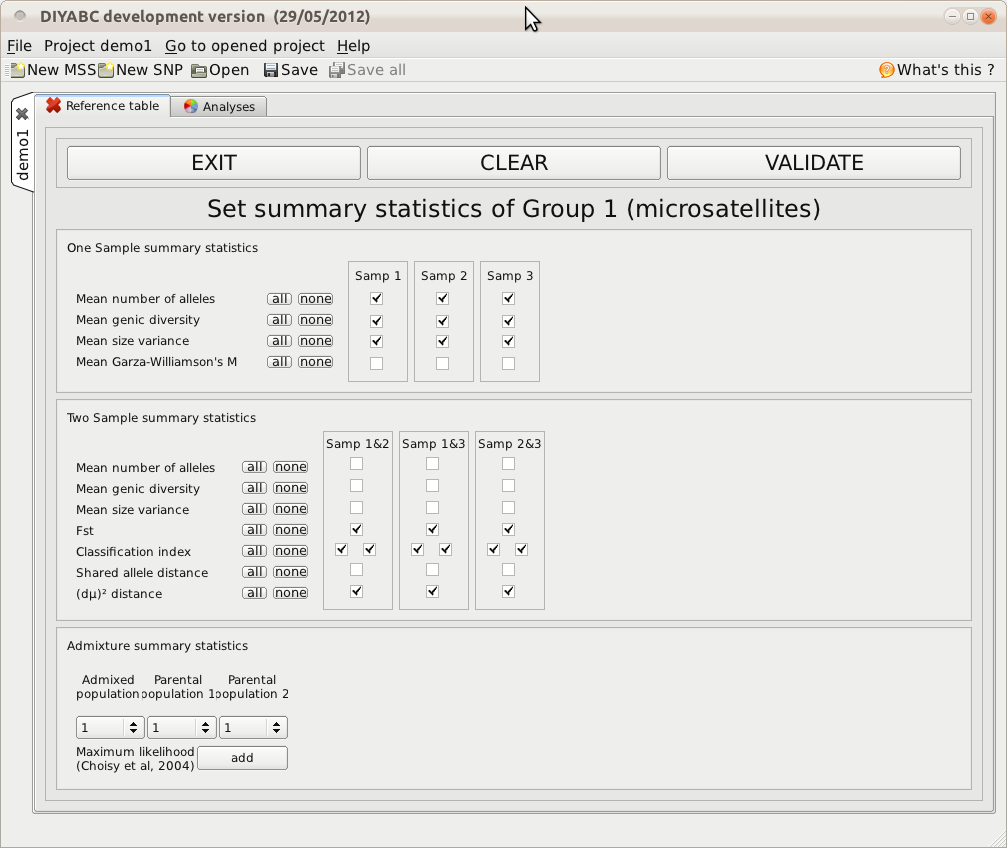
\includegraphics[scale=0.35]{gui_pictures/Capture-DIYABC-21.png} 

Once finished, we click on the \fbox{\textsf{VALIDATE}} button to go back to the screen of p24. Now, we can validate also this screen which brings us back to the screen of p22. The latter looks now like this : \\

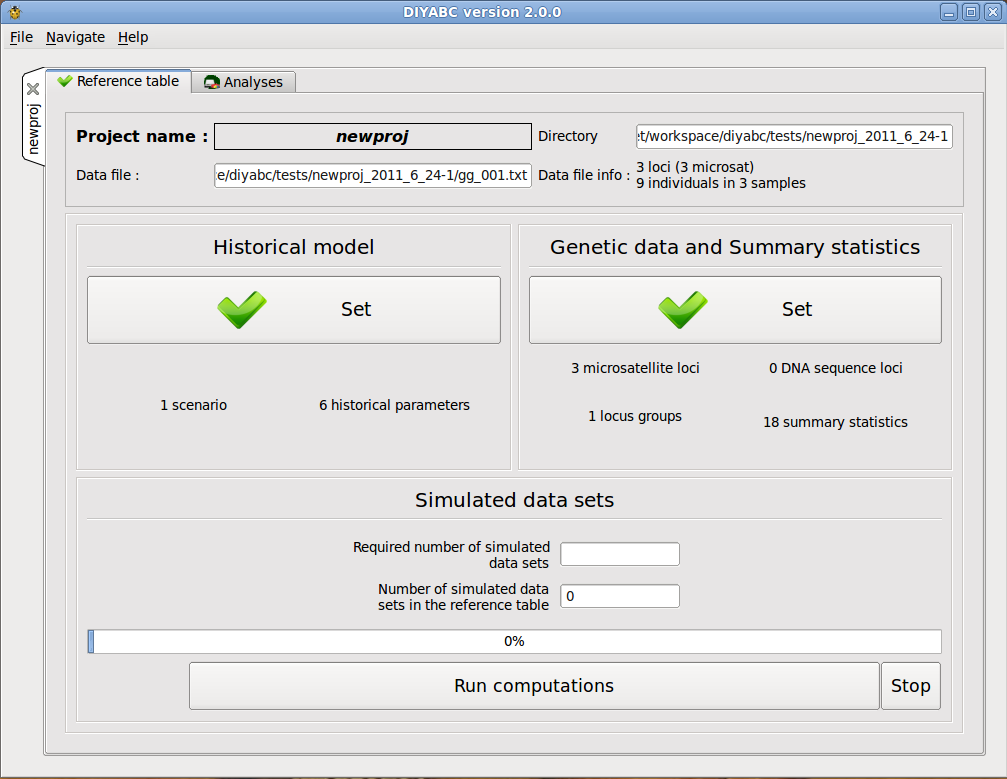
\includegraphics[scale=0.35]{gui_pictures/Capture-DIYABC-22.png} 

At that moment, the project directory includes the following files : a copy of the data file, and four configuration files : \texttt{conf.analysis}, \texttt{conf.gen.tmp}, \texttt{conf.hist.tmp}, \texttt{conf.tmp}. Note that the project is not yet saved. To save the project, we need either to save it explicitly by using the \texttt{File} menu (see below) or to start simulating data sets (next section). Saving the project results in saving the \texttt{header.txt} file in the project directory.


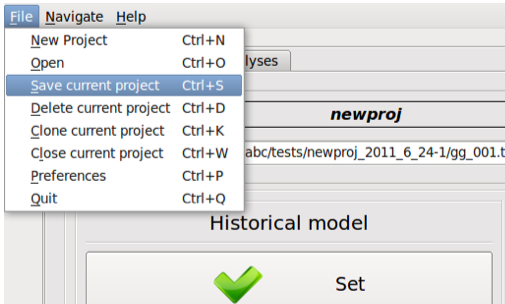
\includegraphics[scale=0.35]{gui_pictures/Capture-DIYABC-23.png} 

\subsection{Building the reference table}

Keeping on the current screen, indicate the required number of data sets to simulate for the reference table : \\ 

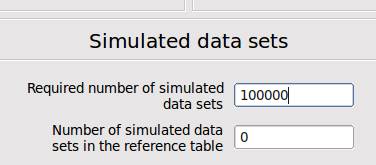
\includegraphics[scale=0.35]{gui_pictures/Capture-DIYABC-24.png} 


Then click on the \fbox{\textsf{Run computations}} button. If things go well, you will soon see the progress both into the edit window "Number of simulated data sets in the reference table" and in the progress bar below. Also, you have an estimate of the remaining time (at the left of the  \fbox{\textsf{Run computations}} button):\\

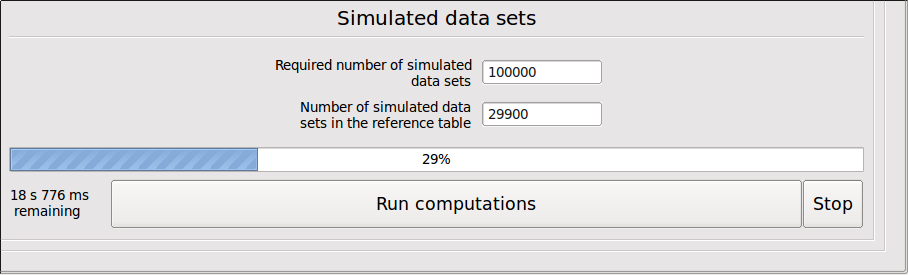
\includegraphics[scale=0.35]{gui_pictures/Capture-DIYABC-25.png} 

When the computation is finished, the screen looks like this :\\

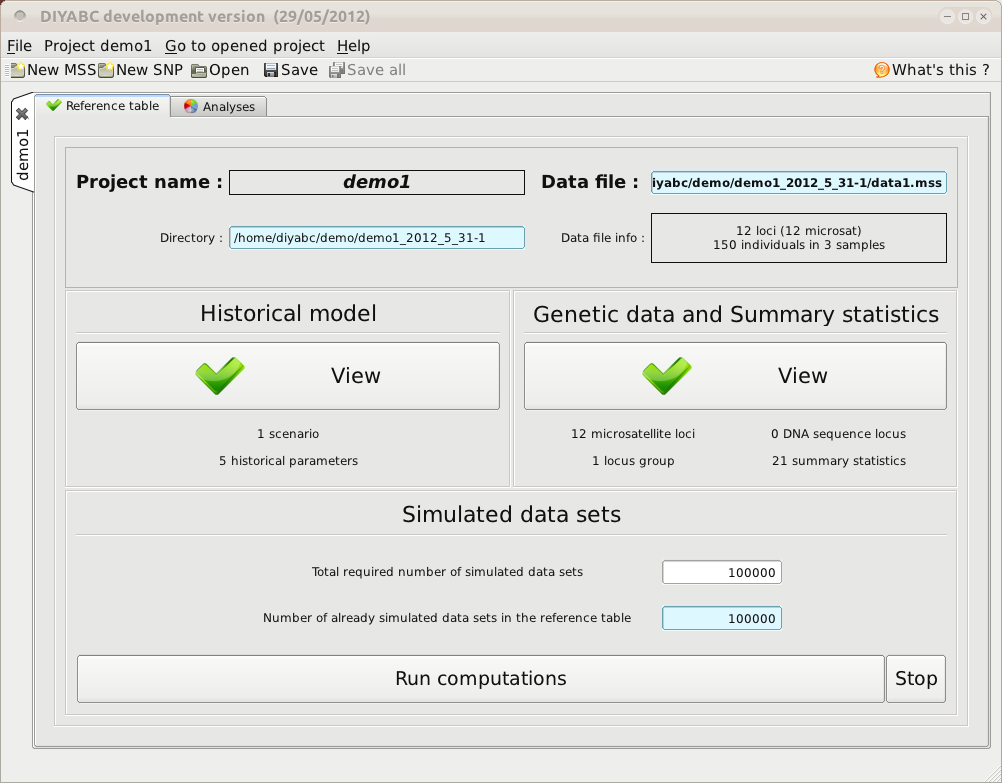
\includegraphics[scale=0.35]{gui_pictures/Capture-DIYABC-26.png} 

\subsection{Performing analyses}

We have now eveything necessary to perform analyses. The current screen shows two tabs : \texttt{Reference table} and \texttt{Analyses}. Let's click on the \texttt{Analyses} tab. We get this new screen :\\

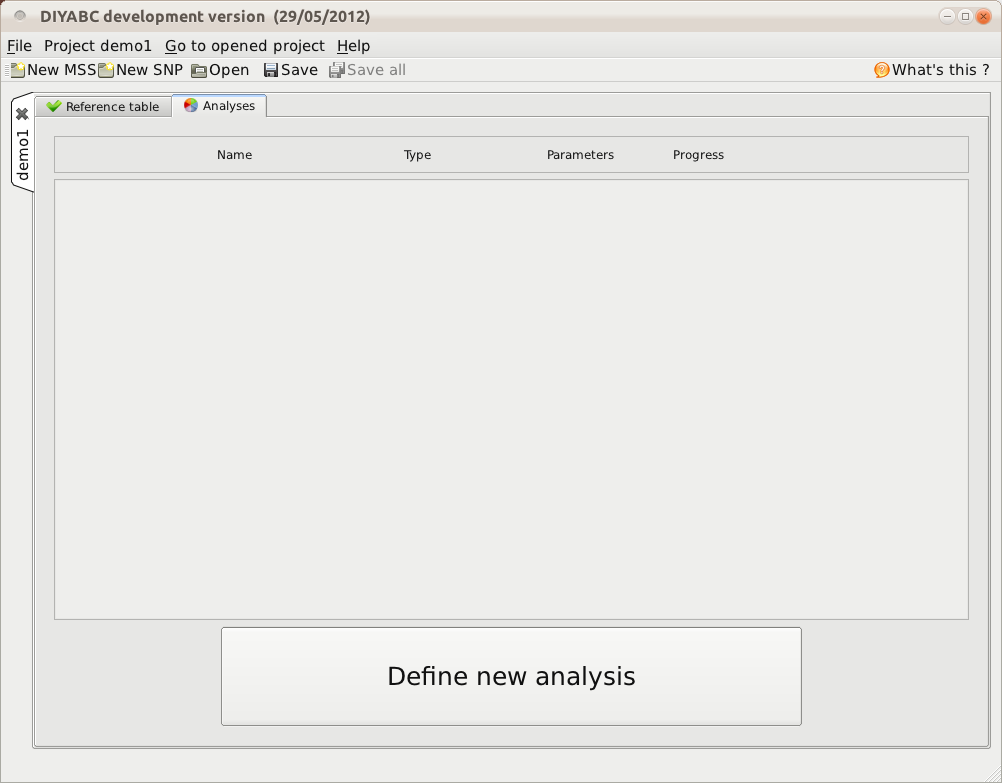
\includegraphics[scale=0.35]{gui_pictures/Capture-DIYABC-27.png} 

First, we need to define the analysis we want to perform. So we click on the \fbox{\textsf{Define new analysis}} button and get this new screen :\\

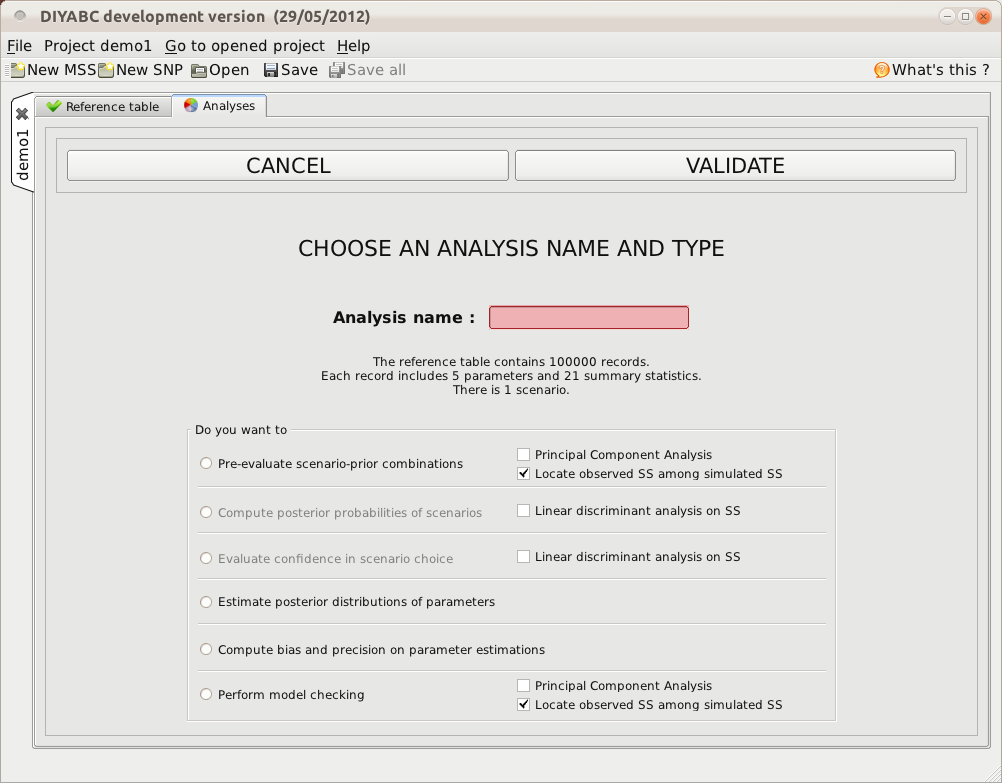
\includegraphics[scale=0.35]{gui_pictures/Capture-DIYABC-28.png} 

We need to choose among the six possible types of analyses (actually, only four of them are possible, since the reference table includes a single scenario). We decide to first check whether the model (scenario and parameter prior definition) is off the target or not. This can be appreciated through the analysis denominated \texttt{Pre-evaluate scenario prior combination}. To illustrate the result, we also ask for a principal component analysis by checking the corresponding square. Eventually, we give the name of \textbf{pre-eval1} to this first analysis. The screen now looks like this :\\

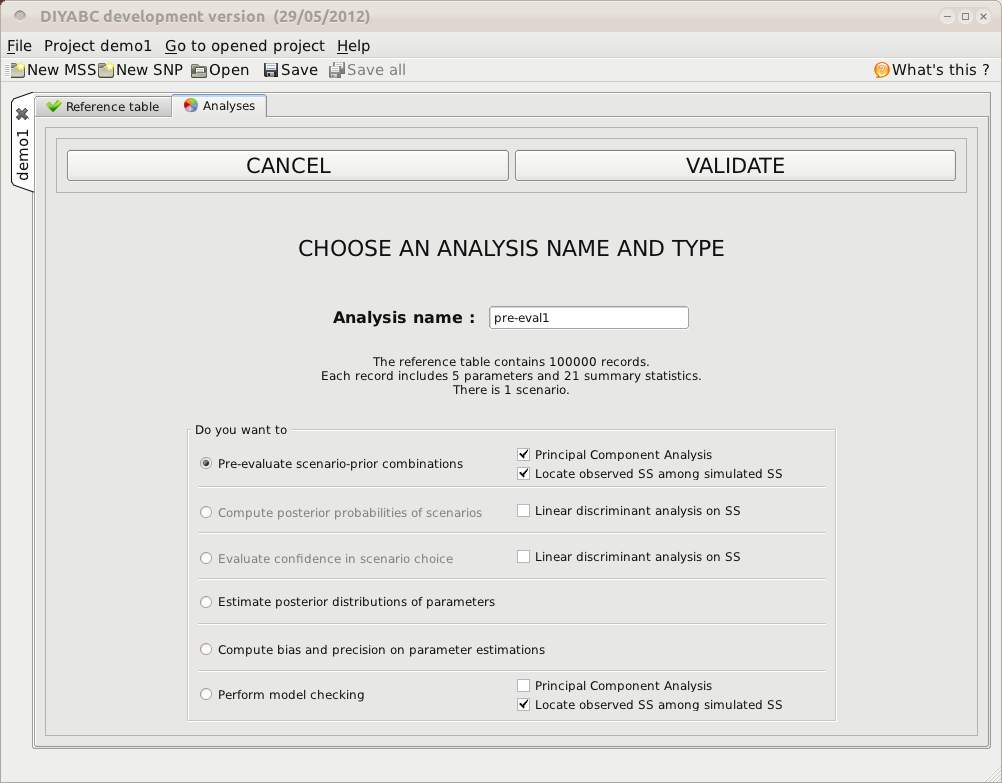
\includegraphics[scale=0.35]{gui_pictures/Capture-DIYABC-29.png}\\ 

After clicking on the \fbox{\textsf{VALIDATE}} button, we go back to the previous screen. However, the new analysis now appears on top of the analysis panel. For each analysis, this panel provides its name and type, the list of parameters that will be transmitted (in a coded way) to the computation program, a progress bar that approximates the progress of the analysis run, and four buttons. The right button has to be clicked to launch the analysis. The three left buttons provide a way to copy an analysis (\fbox{\textsf{Copy}} button), to make some modifications (\fbox{\textsf{Edit}} button) before launching it or to delete the analysis (\fbox{\textsf{Del}} button).\\
 

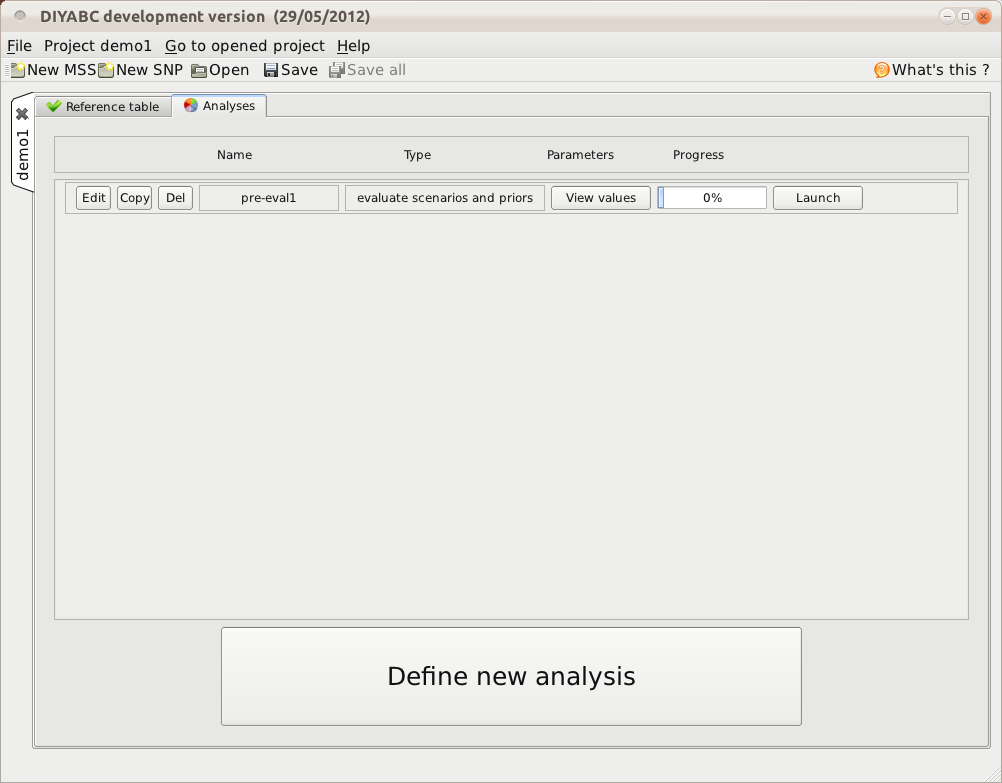
\includegraphics[scale=0.35]{gui_pictures/Capture-DIYABC-30.png} \\

Let's click on the \fbox{\textsf{Launch}} button. This analysis is very fast (ca 1 second) so that the progress bar shows almost immediately a 100\% value : \\

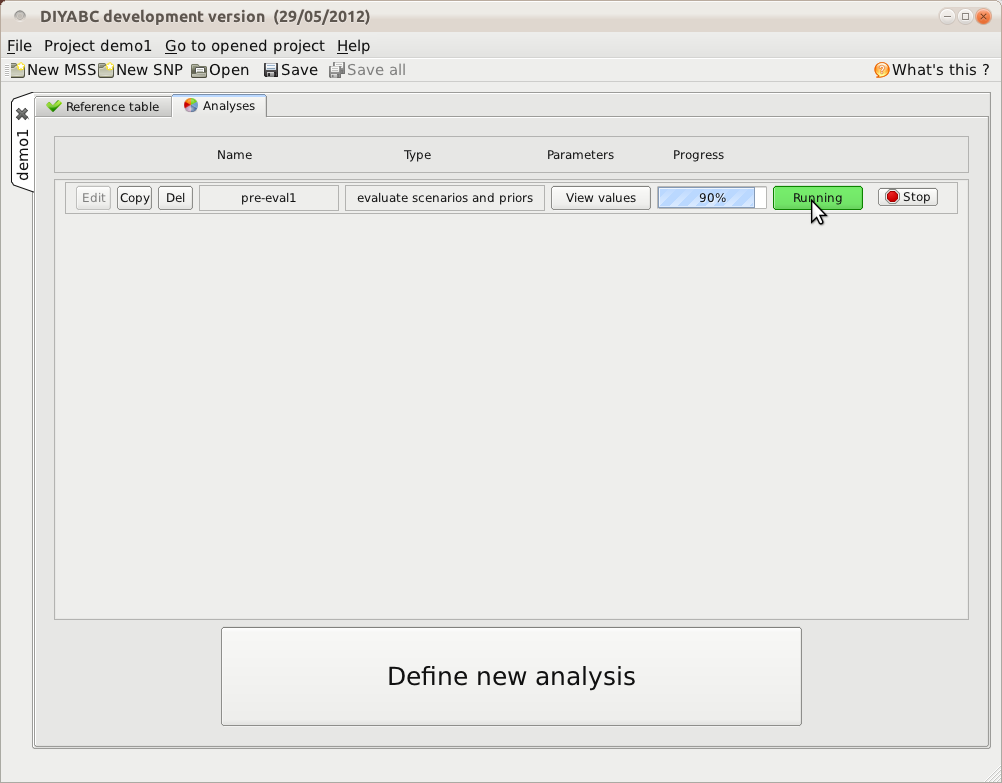
\includegraphics[scale=0.35]{gui_pictures/Capture-DIYABC-31.png} \\

To view results, just click on the \fbox{\textsf{View results}} button. After some seconds (while the program reads the PCA result file), we can see this : \\

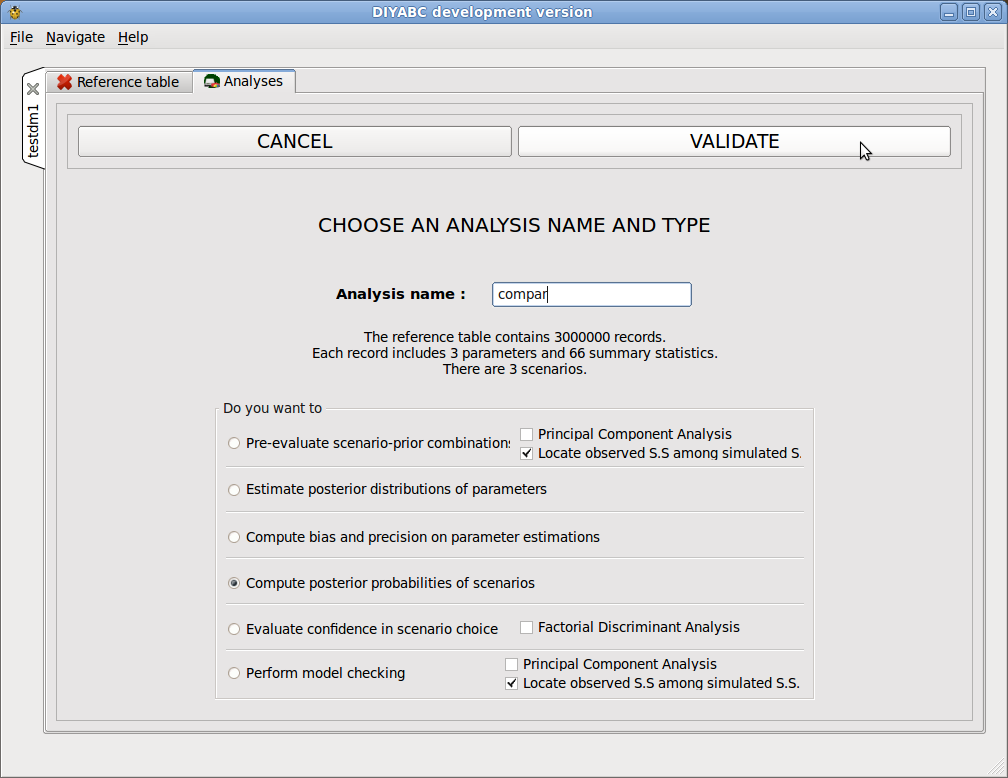
\includegraphics[scale=0.35]{gui_pictures/Capture-DIYABC-32.png} \\

The results are shown PCA plane by PCA plane. Each (small) dot represents a simulated dataset from the reference table and the large yellow dot represents the observed data set. The initial components of datasets are the values of the summary statistics from which are computed the principal components. The four drop-lists (\texttt{Scenario to draw}, \texttt{Horizontal axis component}, \texttt{Vertical axis component}, \texttt{Number of prior plots per scenario}) can be used to explore further the results of the PCA.\\
The graphic can be printed or saved (\fbox{\textsf{PRINT}} and \fbox{\textsf{SAVE}} buttons, respectively). Clicking on the \fbox{\textsf{CLOSE}} button closes the result window. Eventually, clicking on the \fbox{\textsf{View numerical results}} opens up another screen as shown below :\\

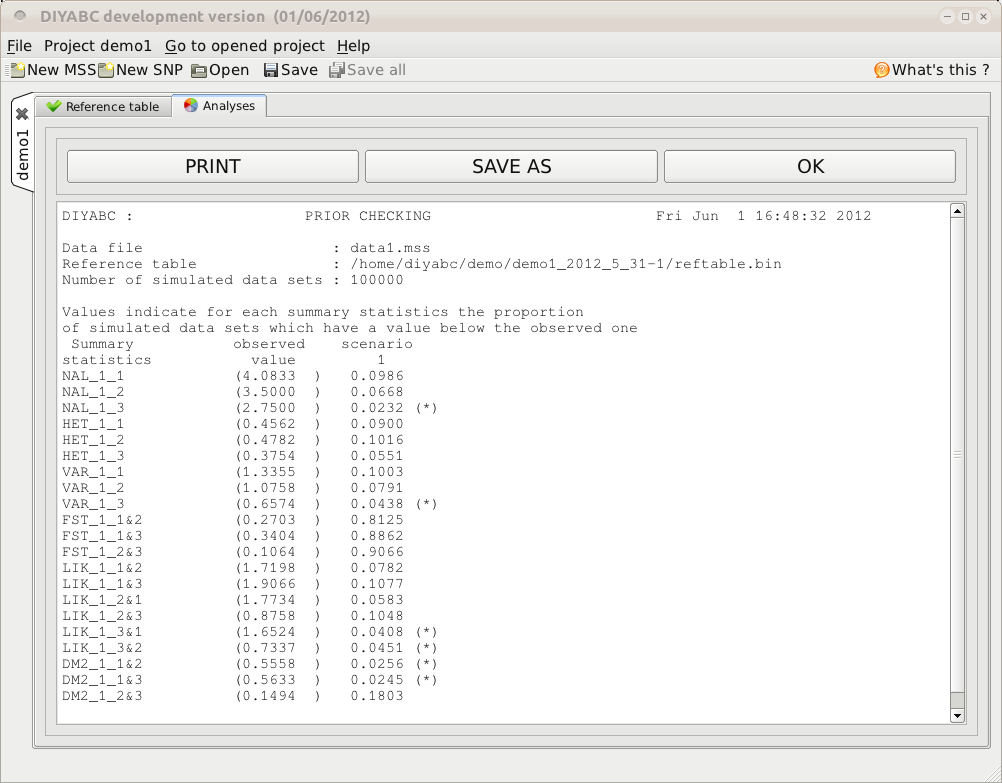
\includegraphics[scale=0.35]{gui_pictures/Capture-DIYABC-33.png} \\

This screen is obtained by computing for each summary statistics the proportion of simulated data (considering the total reference table) that have a value below the value of the observed dataset. A star indicates proportions lower than 5\% or greater than 95\% (two stars, $<$1\% or $>$1\%; three stars, $<$0.1\% or $>$0.1\%).\\ 

 As usual, results can be printed (\fbox{\textsf{PRINT}}) and/or saved (\fbox{\textsf{SAVE}}). Click on \fbox{\textsf{OK}} to leave this screen.\\

Although we get one star for a few summary statistics, we conclude that our model is suitable enough to proceed to other ABC analyses.

\subsubsection{ABC parameter estimation}

Back on the screen of page 30, we click on the \fbox{\textsf{Define new analysis}} button. We choose the \texttt{Estimate posterior distribution of parameters} option and we call \texttt{estim1} this second analysis :\\

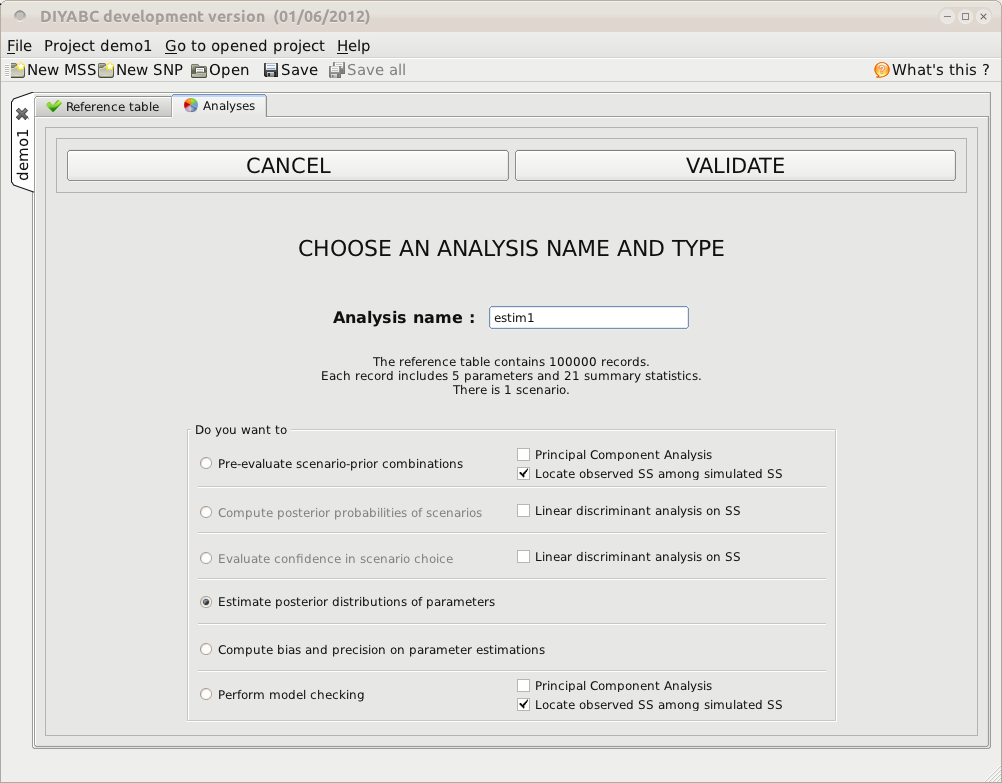
\includegraphics[scale=0.35]{gui_pictures/Capture-DIYABC-34.png} \\
 
We click on the \fbox{\textsf{VALIDATE}} button and get the following screen in which we can choose the scenario to use for this estimation. Since a single scenario has been defined, there is nothing else to do than to click on the \fbox{\textsf{VALIDATE}} button : \\

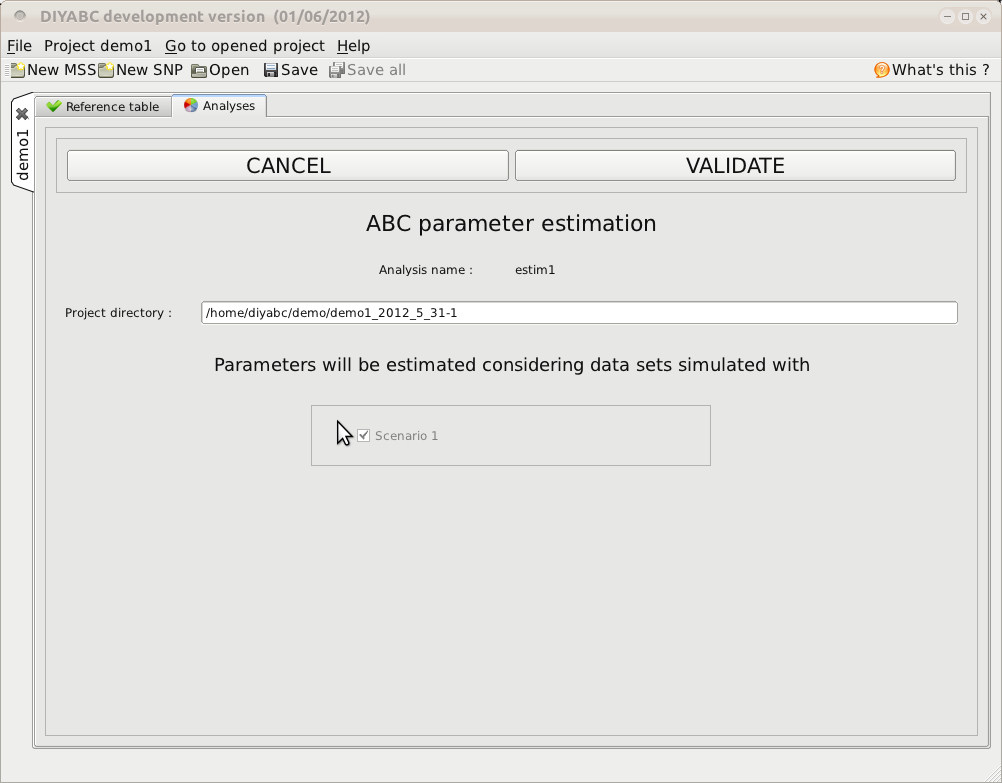
\includegraphics[scale=0.35]{gui_pictures/Capture-DIYABC-35.png} \\
 
We get then the following screen in which we can make several choices :
\begin{itemize}
 \item on the left hand side, we can choose the number of closest simulated datasets that will be used for the local linear regression (cf section 2.1).
 \item below, we can select the transformation of parameter values that can generally improve the results (default = logit transformation).
 \item on the right hand, we can truncate the reference table to a specified number of datasets.
 \item eventually, estimations can be performed either on original ($i.e.$ raw) parameters, and/or combinations of parameters that are generally more estimable. \emph{Composite} parameters are products of effective population sizes or times by mean mutation rate whereas \emph{Scaled} parameters are ratios of effective population sizes or times by mean effective population size (computed from all terminal populations, $i.e.$ $N_1$, $N_2$ and $N_3$ in the present example). 
\end{itemize}

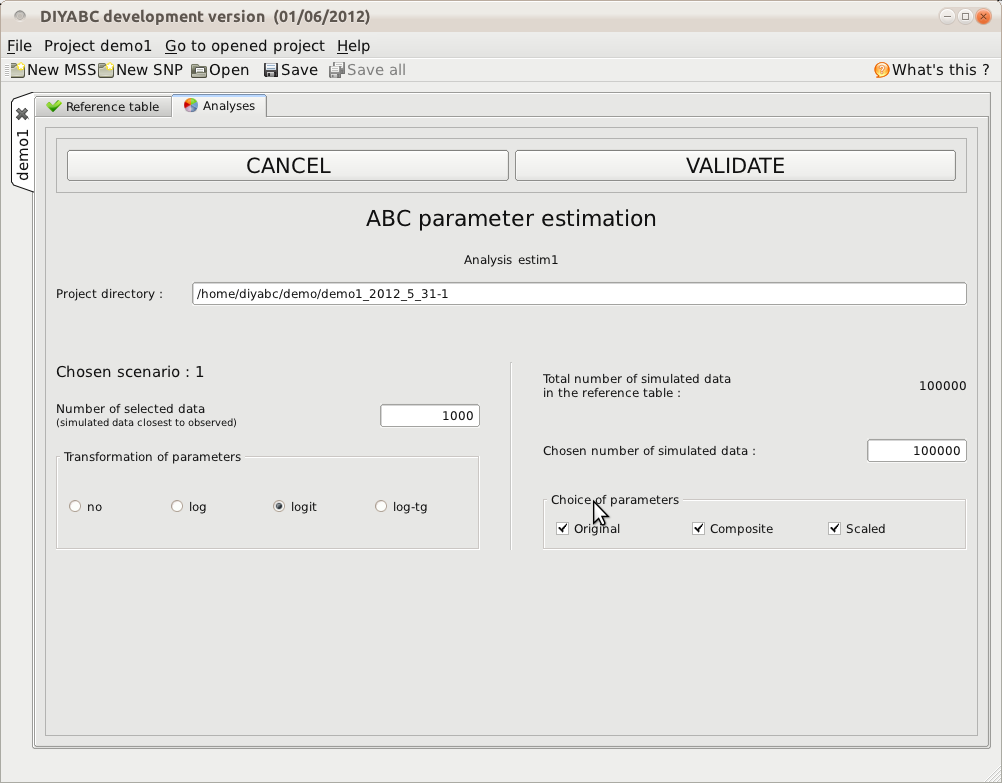
\includegraphics[scale=0.35]{gui_pictures/Capture-DIYABC-36.png} \\
 
Apart from the number of closest datasets that we set at 10,000 (although 1,000 would be also a correct choice), we keep all other default values and click on the \fbox{\textsf{VALIDATE}} button. We get back to the Analysis control panel which now looks like this:\\

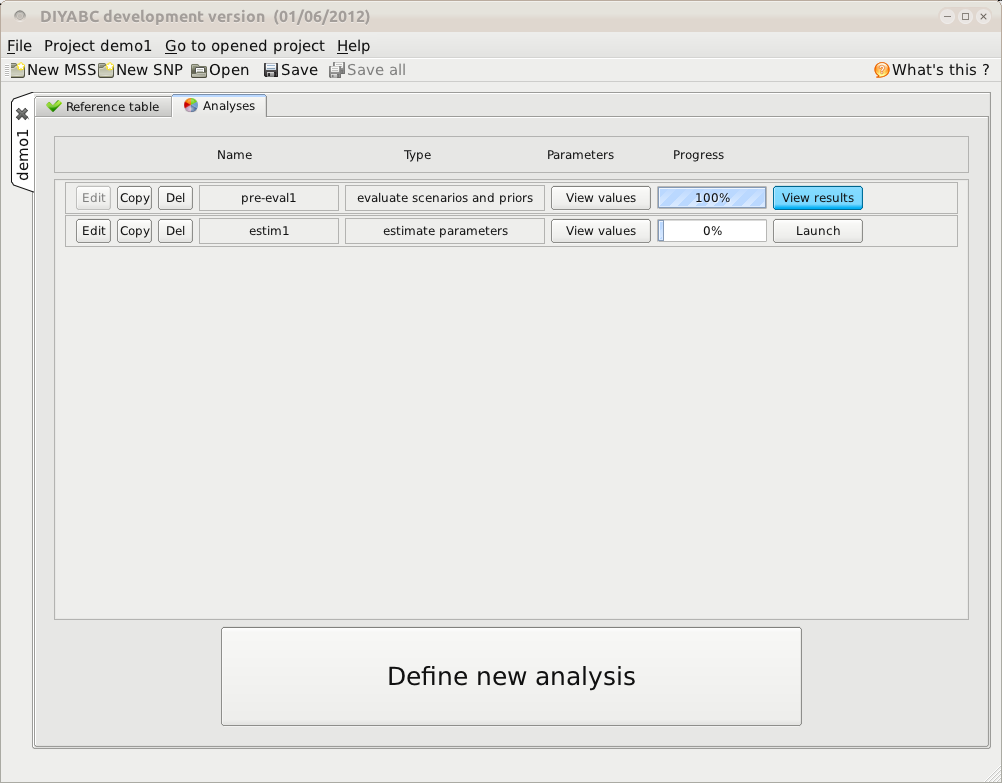
\includegraphics[scale=0.35]{gui_pictures/Capture-DIYABC-38.png} \\

%\newpage
We click on the \fbox{\textsf{Launch}} button. The analysis progress is now visible :\\

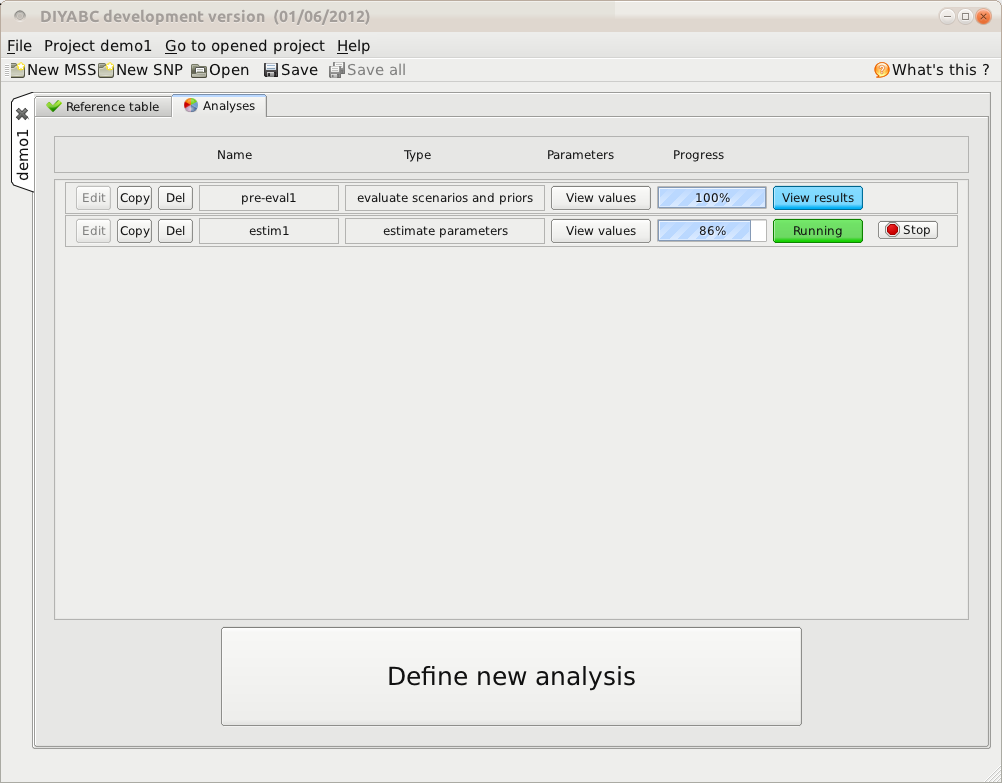
\includegraphics[scale=0.35]{gui_pictures/Capture-DIYABC-38a.png} \\

As long as the analysis is not terminated, we could stop it by clicking on the  \fbox{\textsf{Stop}} button. Once this second analysis is finished, we can view its results by clicking on the  \fbox{\textsf{View results}} button :\\

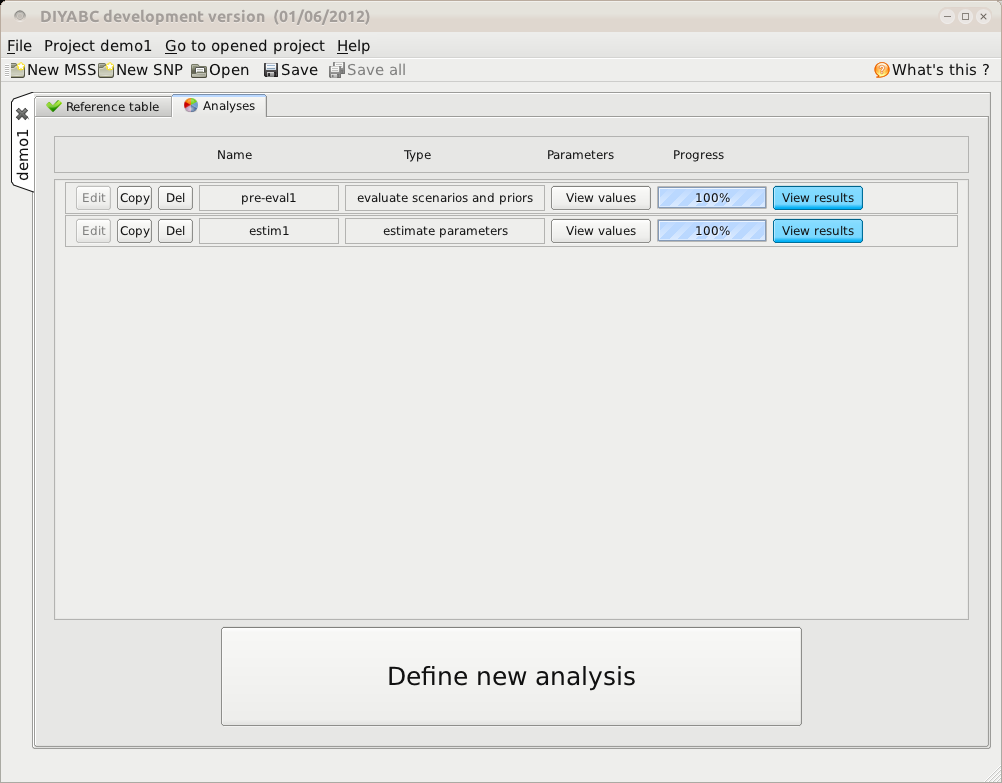
\includegraphics[scale=0.35]{gui_pictures/Capture-DIYABC-39.png} \\

Let's have a look :\\

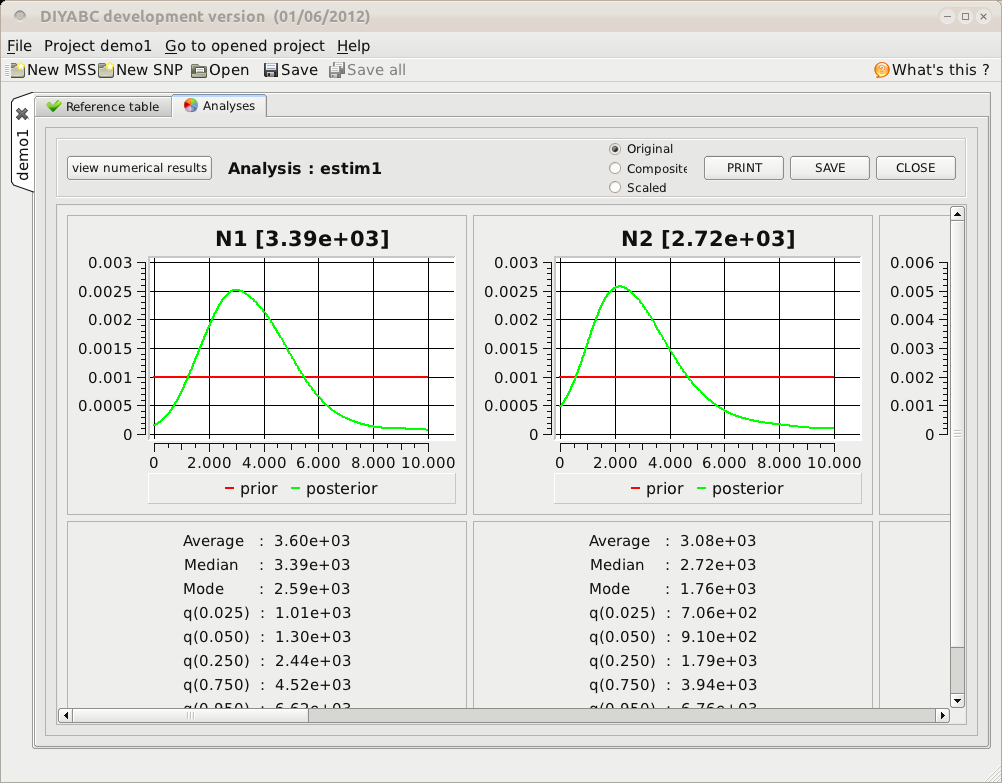
\includegraphics[scale=0.35]{gui_pictures/Capture-DIYABC-40.png} \\

In the scrolling window, we get graphics showing the prior (red curve) and posterior (green curve) distributions of all parameters. Below each graphics are statistics (mean, median, mode and quantiles) of the posterior distribution. The latter are grouped in a table that appears when clicking on the upper left \fbox{\textsf{view numerical results}} button, showing this :\\

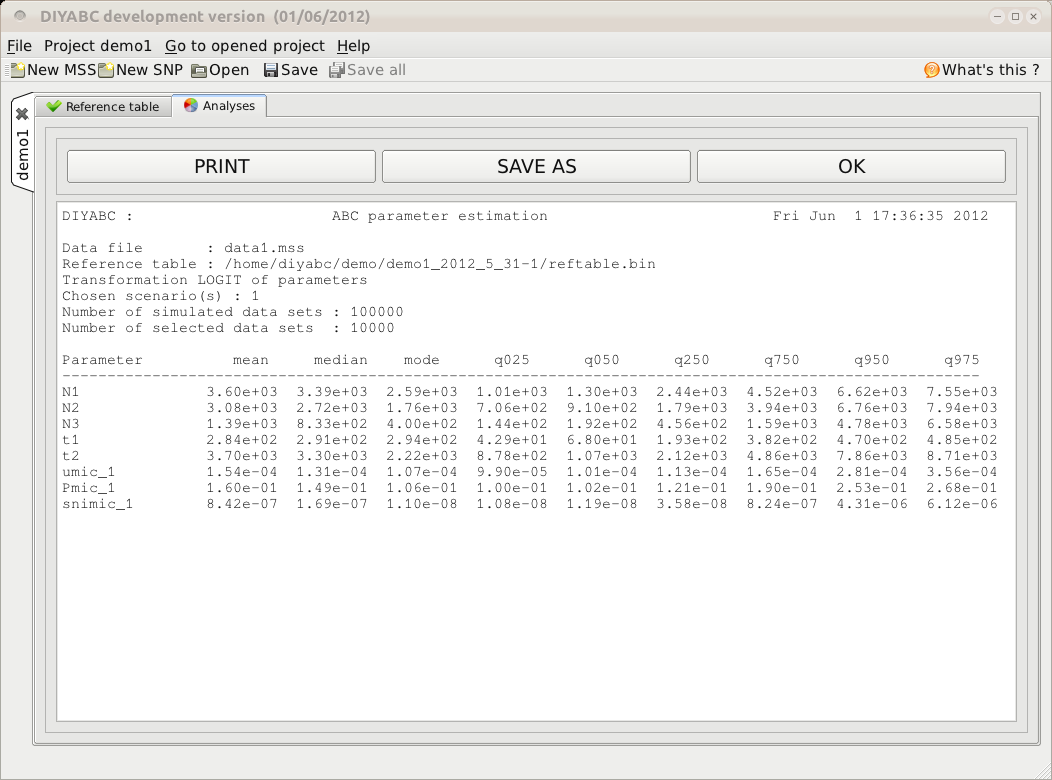
\includegraphics[scale=0.35]{gui_pictures/Capture-DIYABC-41.png} \\

We go back to the previous screen by cliking the \fbox{\textsf{OK}} button.
\newpage
 We can also have results for \emph{Composite} or \emph{Scaled} parameters. Below is an example of \emph{Scaled} time parameters obtained by clicking on the \emph{Scaled} radio button and scrolling the graphs window to the right:\\
 
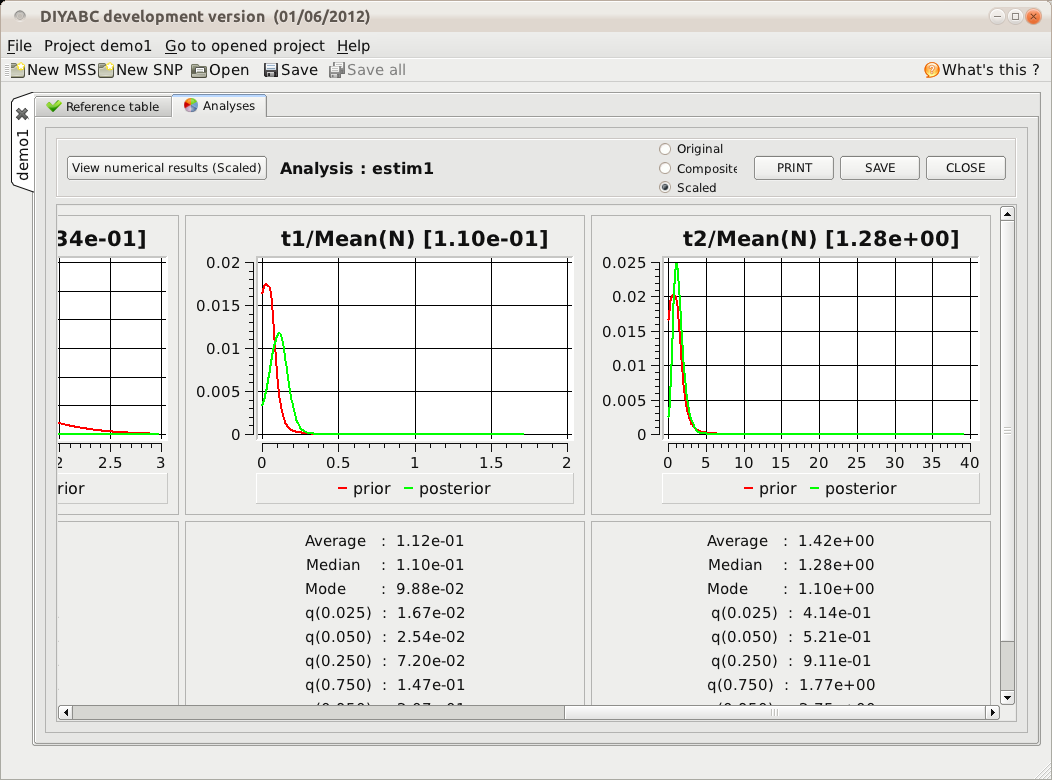
\includegraphics[scale=0.35]{gui_pictures/Capture-DIYABC-42.png} \\


\subsubsection{Bias and precision}
Let's define a new analysis (click on the \fbox{\textsf{Define new analysis}} button) and choose the option \texttt{Compute bias and precision on parameter estimations}. We give it the name \texttt{bias1} :\\

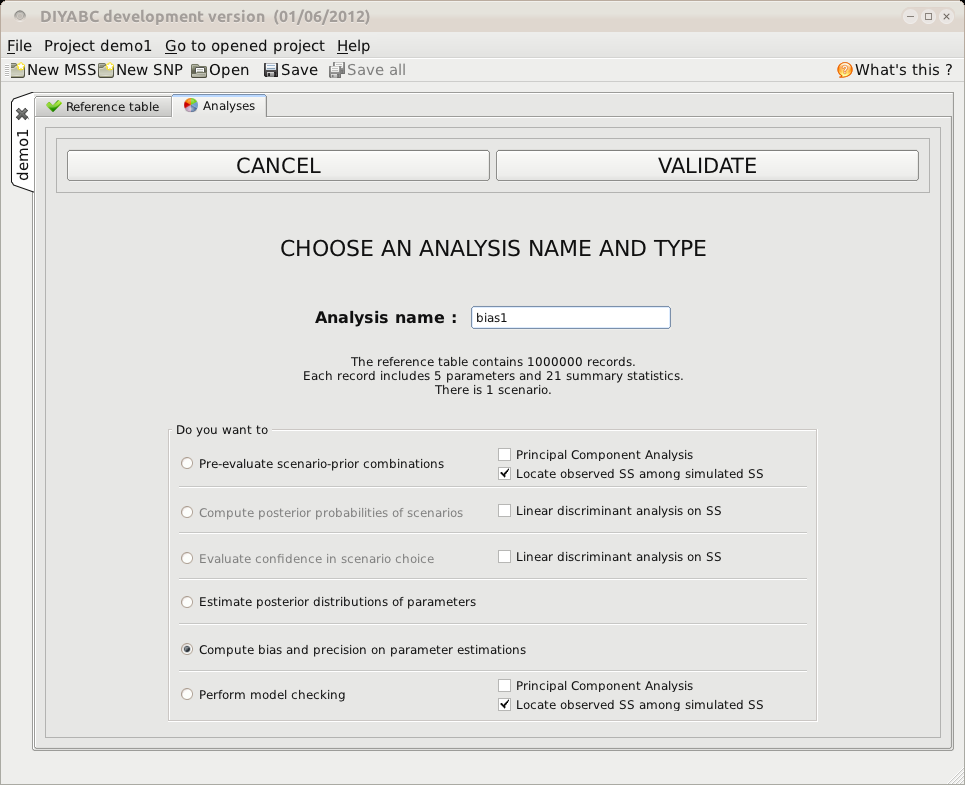
\includegraphics[scale=0.35]{gui_pictures/Capture-DIYABC-43.png} \\

In this kind of analysis, peudo-observed data are simulated with known values of parameters copying the exact configuration of the observed dataset in terms of sample sizes (taking into account missing data) and are submitted to the same ABC estimation process. If we assume that the evolutionary scenario is correct, the comparison of real and estimated values of parameters provide some information of the precision of the estimation process.\\  
We validate and get this screen :\\

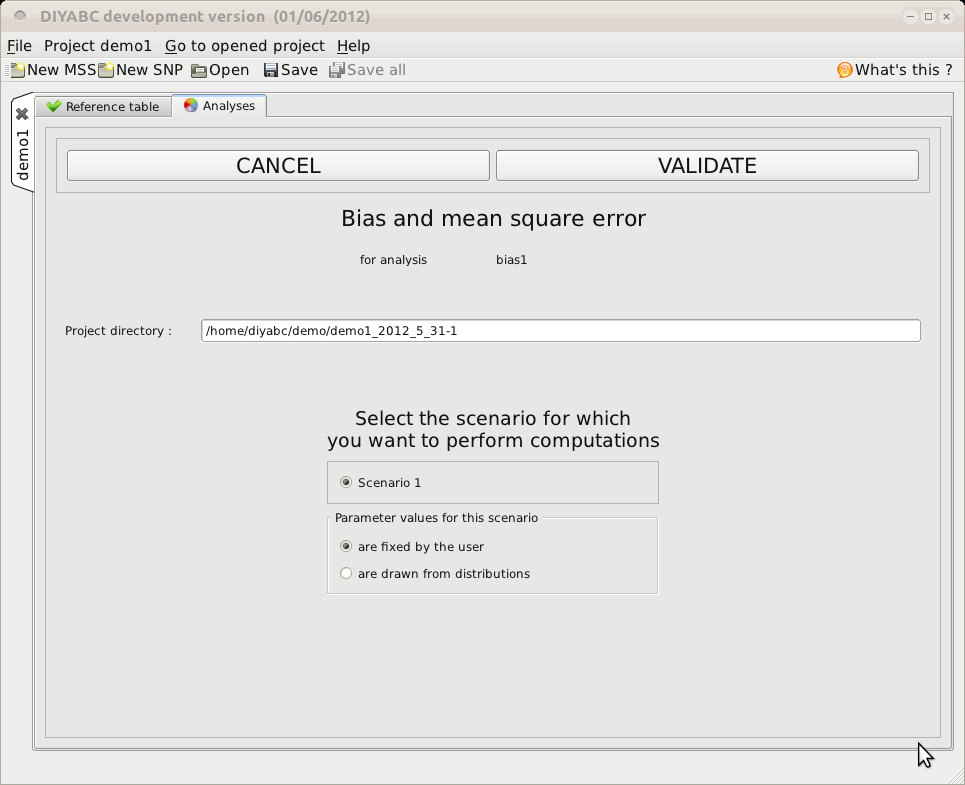
\includegraphics[scale=0.35]{gui_pictures/Capture-DIYABC-44.png} \\

We choose to draw parameter values from distributions :\\

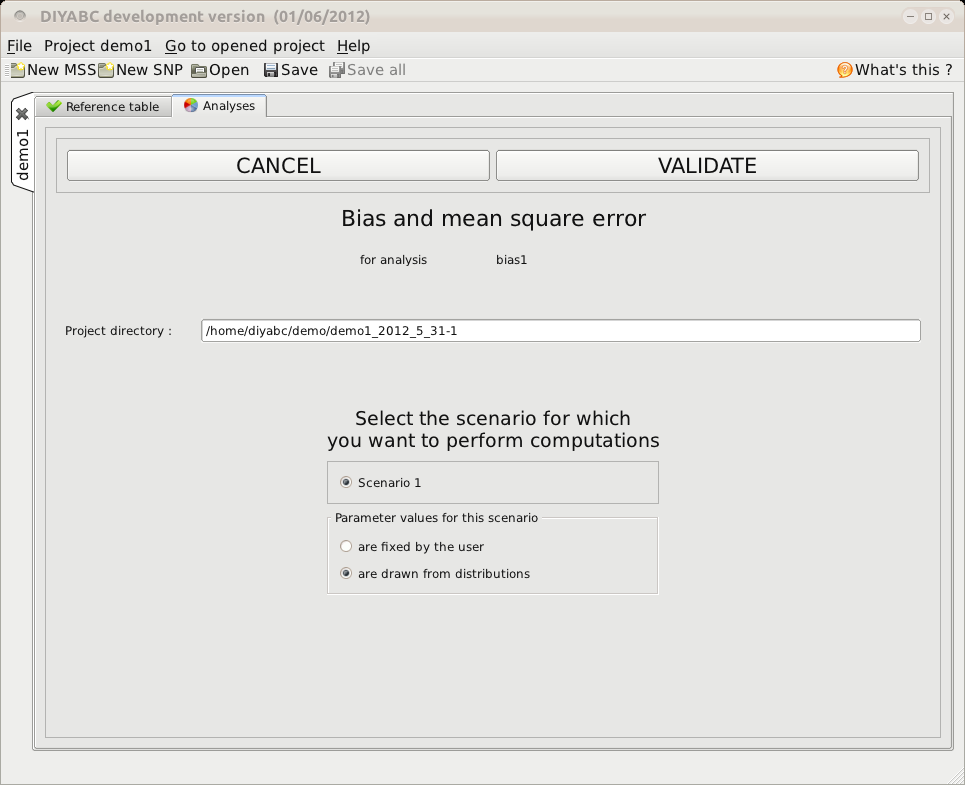
\includegraphics[scale=0.35]{gui_pictures/Capture-DIYABC-45.png} \\

Clicking on the \fbox{\textsf{VALIDATE}} button, we get this screen which allows us to choose distributions. \\

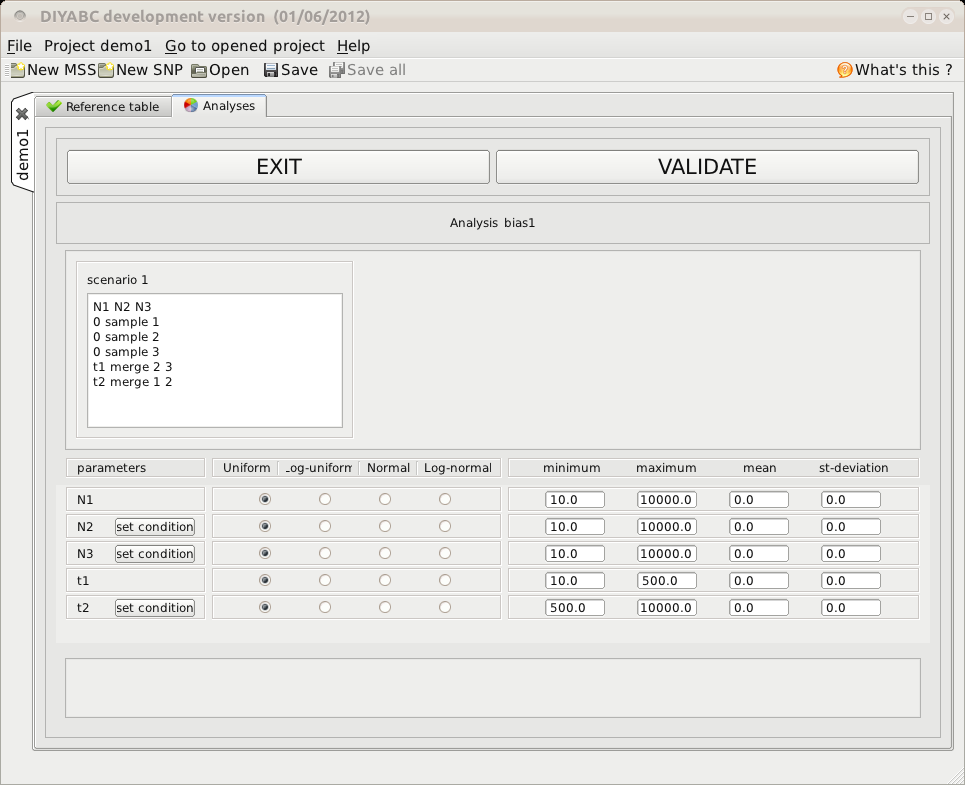
\includegraphics[scale=0.35]{gui_pictures/Capture-DIYABC-46.png} \\

By default, the screen suggests the prior distributions that have been used to build the reference table. However, these distributions can be edited if necessary. We decide not to change them and click on \fbox{\textsf{VALIDATE}} which brings us to the following screen :\\

\includegraphics[scale=0.35]{gui_pictures/Capture-DIYABC-47.png} \\

If we want to keep the same distributions for mutation parameters as when builduing the reference table, we just click on \fbox{\textsf{VALIDATE}}. If we need to change them, we click on \fbox{\textsf{Set mutation model}} which would bring the following screen :\\

\includegraphics[scale=0.35]{gui_pictures/Capture-DIYABC-48.png} \\

After validating twice, we get the last screen necessary to define this king of analysis :\\

\includegraphics[scale=0.35]{gui_pictures/Capture-DIYABC-49.png} \\
 
This screen is similar to that for parameter estimation (see section 3.5.1). After validating, we get back to the analysis panel with a third analysis defined :\\

\includegraphics[scale=0.35]{gui_pictures/Capture-DIYABC-50.png} \\

The analysis takes some time to run compared to the previous one, because it simulates hundreds datasets and on each one, a full ABC estimation is performed. Then after some time, the analysis is finished: \\

\includegraphics[scale=0.35]{gui_pictures/Capture-DIYABC-51.png} \\

To view results, we click on the  \fbox{\textsf{View results}} button. 

\newpage

The results are visible in a scrolling window :\\

\includegraphics[scale=0.32]{gui_pictures/Capture-DIYABC-52a.png} \\

Note that there are two values given for each statistics. The upper value is that of the statistics computed from the \emph{posterior} distribution of parameters, $i.e.$ \textbf{using the genetic information provided by data}. The lower value, noted between parentheses, is that of the statistics computed from the \emph{prior} distribution of parameters, $i.e.$ \textbf{NOT using the genetic information provided by data but only that contained in prior distributions}.  

\subsubsection{Model Checking}
We now define another type of analysis called \texttt{Model Checking} which is used to evaluate how well the scenario and priors of parameters fit the data summarized by summary statistics. This is the last option on the following screen :\\

\includegraphics[scale=0.32]{gui_pictures/Capture-DIYABC-53.png} \\

We call this analysis \texttt{mc1} and check the box to get a PCA performed. This PCA is computed in the same way compared to that of the first option (\texttt{Pre-evaluate scenario prior combinations}). However, new datasets simulated with parameters drawn from the posterior distributions of parameters are also represented on the different planes of the PCA (but not taken in the PCA  computation). 

We validate the above screen and get the usual next screen :\\

\includegraphics[scale=0.35]{gui_pictures/Capture-DIYABC-54.png} \\

that we just validate to get the last screen :\\

\includegraphics[scale=0.35]{gui_pictures/Capture-DIYABC-55.png} \\

In this screen which we have already seen, there is a new panel (bottom right) in which we can choose the number of datasets that we want to simulate from the posterior distributions of parameters. There is also a button  \fbox{\textsf{Redefine summary statistics of group:}} shown by the pointer. This button allows to change the set of summary statistics (for a given group of loci chosen through the drop list on the right). Clicking on this button opens up the usual following screen in which, by default, are checked the summary statistics in the reference table.\\

\includegraphics[scale=0.35]{gui_pictures/Capture-DIYABC-56.png} \\

We decide to use all one-sample and two-sample summary stats :\\

\includegraphics[scale=0.35]{gui_pictures/Capture-DIYABC-57.png} \\
 

Note that when the set of summary statistics is changed (as here), it is necessary to also simulate a large number of datasets using parameter priors to get corresponding values of the newly introduced summary statistics. We validate twice and launch the analysis. When it is finished, we click on the  \fbox{\textsf{View results}} button and get this screen:\\

\includegraphics[scale=0.33]{gui_pictures/Capture-DIYABC-58.png} \\

Clicking on the \fbox{\textsf{View numerical results}} leads to the following screen which provides, for each individual summary statistics, the value in the observed dataset as well as the proportion of data sets (simulated from the posterior) that have a value lower than the observed data set.\\
 
\includegraphics[scale=0.33]{gui_pictures/Capture-DIYABC-60.png} \\


Notice that in this computation, values that are in the interval $[s_{obs}-0.001,s_{obs}+0.001]$ are counted for one half those that are outside the interval. This explains why the fourth digit of the proportion can be 0 or 5 while having simulated 1000 data sets.\\
Here the conclusion is that the chosen model/posterior explain correctly the observed dataset (see \cite{C2010} for further illustrations). 

\subsubsection{Posterior probabilities of scenarios}
Consider a new example dataset in which three populations have been sampled. We want to decide which scenario is the best supported by data, a divergence scenario (scenario 1) or a split scenario (scenario 2) :\\

\includegraphics[scale=0.33]{gui_pictures/Capture-DIYABC-113.png} \\

Suppose that we have already built a reference table with these two scenarios. We define a new analysis that we call \texttt{comp1} :\\

\includegraphics[scale=0.33]{gui_pictures/Capture-DIYABC-105.png} \\
 
Note here that it is possible to replace original summary statistics (SS) by discriminant scores by checking the box \texttt{Linear discriminant analysis on SS}. This option is useful when there are numerous scenarios and many summary statistics \citep{EL2012}. However, in the present case, this is not necessary since the analysis with original summary statistics takes only a few seconds. After clicking on the \fbox{\textsf{VALIDATE}} button, we fill in the required fields, taking default values except for the number of local linear regression (on the second screen) that we set to 10:\\

\includegraphics[scale=0.3]{gui_pictures/Capture-DIYABC-109.png} \\

So that we get the following screen :\\

\includegraphics[scale=0.3]{gui_pictures/Capture-DIYABC-110.png} \\

After validating the screen above, we launch the analysis which lasts a few seconds and press on the \fbox{\textsf{View results}} button. The following screen appears:\\

 \includegraphics[scale=0.3]{gui_pictures/Capture-DIYABC-111.png} \\

Both analyses agree that scenario 1 is the best supported scenario in this comparison. If we click on the \fbox{\textsf{View numerical results}}, the program shows a subset of numerical values used in the previous screen (i.e. the probability values with their 95\% confidence intervals for the 10 subsets of closest simulated data). Note that the 95\% CIs can be used to ensure that probabilities are significantly different among scenarios.\\

 \includegraphics[scale=0.3]{gui_pictures/Capture-DIYABC-112.png} \\

\subsubsection{Confidence in scenario choice}

This last type of analysis is aimed at evaluating with which level of confidence we can trust the previous analysis. To do so, we simulate new datasets with each scenario, apply the same procedure for estimating their respective posterior probabilities and measure the proportion of times the right scenario has the highest posterior probability.\\
We then define a new analysis, \texttt{conf1} as below:\\   

\includegraphics[scale=0.33]{gui_pictures/Capture-DIYABC-115.png} \\

As for the previous analysis, it is possible to replace original summary statistics by discriminant scores. This is still more useful here since this type of analysis can last hours. However, with our current example, the analysis will not last more than a few minutes.\\
The next screen (below) needs some editing :\\

\includegraphics[scale=0.33]{gui_pictures/Capture-DIYABC-116.png} \\

We check the two scenario boxes on the right and decide to simulate datasets according to priors :\\

\includegraphics[scale=0.38]{gui_pictures/Capture-DIYABC-117.png} \\

After validating default values for historical and mutational parameters, we launch the analysis. When it is done, we click on the \fbox{\textsf{View results}} button and get the following screen:\\

\includegraphics[scale=0.38]{gui_pictures/Capture-DIYABC-119.png} \\

At the bottom, there is a summary of results, $i.e.$ the number of times each scenario has the highest posterior probability under each approach:\\

\includegraphics[scale=0.33]{gui_pictures/Capture-DIYABC-120.png} \\

We can deduce the type I error for scenario 1,  which is the probability with
which it is rejected although it is the true scenario : 20 using the direct
method (or 19 using the regression method) over 500, $i.e.$ 0.04 (0.038). To
have access to the type II error (probability of deciding for scenario 1 when it
is not the true scenario), we need to run the same analysis but simulating
according to all other scenarios (only scenario 2 in the present example) and
counting decisions in favor of scenario 1. Running the example analysis with
scenario 2 gives 77 (or 36) over 500 in favor of scenario 1. This gives an
estimate of type II error of 0.154 (0.072) for scenario 1.

\subsection{Simulating data sets}

The $DIYABC$ program can also be used to simulate data sets, either microsatellite and/or DNA sequence data sets using our Genepop format, or SNP data sets using our specific format. This option is reachable through the main \textsf{File} menu as shown below :\\

\includegraphics[scale=0.33]{gui_pictures/Capture-DIYABC-62.png} \\

Clicking on e.g. the \textsf{Microsatellites and/or sequences (Genepop format)} opens up a dialog window in which one can choose the directory into which will be located the project and the future data files :\\

\includegraphics[scale=0.33]{gui_pictures/Capture-DIYABC-64.png} \\

Above, we decided to call \textsf{demo2} this new directory and to locate it in the \textsf{home/diyabc/demo} directory.

Clicking on \fbox{\textsf{OK}} leads to usual screen:\\

\includegraphics[scale=0.33]{gui_pictures/Capture-DIYABC-65.png} \\

We first inform the historical model clicking on the  \fbox{\textsf{Set}} button under \textsf{Historical model}. We edit the scenario box as below:\\

\includegraphics[scale=0.33]{gui_pictures/Capture-DIYABC-66.png} \\

We click on the  \fbox{\textsf{Set parameter values}} button. Arbitrary default values appear :\\

\includegraphics[scale=0.33]{gui_pictures/Capture-DIYABC-67.png} \\

We change these values according to our needs and we click the \fbox{\textsf{Set sample size}} button, getting this screen:\\

\includegraphics[scale=0.33]{gui_pictures/Capture-DIYABC-68.png} \\

We input the needed sample sizes as below :\\

\includegraphics[scale=0.33]{gui_pictures/Capture-DIYABC-69.png} \\

Clicking on the \fbox{\textsf{VALIDATE}} button, we get back to the previous screen showing that the Historical model is now completed:\\

\includegraphics[scale=0.33]{gui_pictures/Capture-DIYABC-70.png} \\


We have now to complete the Genetic data (click on the \fbox{\textsf{Set}} button under \textsf{Genetic data}). The following screen appears:\\

\includegraphics[scale=0.33]{gui_pictures/Capture-DIYABC-71.png} \\

We want a data set including three autosomal, two X-linked and one Y-linked diploid microsatellite loci and one mitochondrial sequence. We also need a sex ratio of one male for four females :\\

\includegraphics[scale=0.33]{gui_pictures/Capture-DIYABC-72.png} \\

We click on the \fbox{\textsf{OK}} button and get the following screen :\\

\includegraphics[scale=0.33]{gui_pictures/Capture-DIYABC-73.png} \\

Our mitochondrial DNA sequence is only 500 nucleotides long and there is a slight excess of A+T (60\%). We edit the corresponding cells : \\

\includegraphics[scale=0.33]{gui_pictures/Capture-DIYABC-74.png} \\

Since mutation models are different for microsatellites and DNA sequences, we define two groups by clicking twice on the \fbox{\textsf{Add group}} button :\\

\includegraphics[scale=0.33]{gui_pictures/Capture-DIYABC-75.png} \\

We select the 6 microsatellite loci by clicking on the first locus name cell and shift-clicking on the sixth locus name cell :\\

\includegraphics[scale=0.33]{gui_pictures/Capture-DIYABC-76.png} \\

The six locus names are transferred into group 1 by clicking on the \fbox{\textsf{$>>$}} button :\\

\includegraphics[scale=0.33]{gui_pictures/Capture-DIYABC-77.png} \\

Then the DNA sequence locus is selected :\\

\includegraphics[scale=0.33]{gui_pictures/Capture-DIYABC-78.png} \\

and transferred into group 2 in the same way :\\

\includegraphics[scale=0.33]{gui_pictures/Capture-DIYABC-79.png} \\

We need now to define the mutation model of each group. Let's click on the \fbox{\textsf{Set Mutation Model}} button of group 1:\\

\includegraphics[scale=0.33]{gui_pictures/Capture-DIYABC-80.png} \\

The usual default values appear. We want to exclude single nucleotide insertions/deletions (SNI mutations). So we set to 0 the Mean SNI rate and Minimum, Maximum and Shape of individual loci SNI rates :\\

\includegraphics[scale=0.33]{gui_pictures/Capture-DIYABC-81.png} \\

Once this done, we go back to the previous screen by clicking on the \fbox{\textsf{VALIDATE}} button. Then we set the mutation model of the mitochondrial DNA sequence. The default values are as follows :\\

\includegraphics[scale=0.33]{gui_pictures/Capture-DIYABC-82.png} \\

The default mean mutation rate is not suited to mitochondrial DNA which generally evolves at a faster rate than nuclear DNA \citep{HL2008}. So we set its value to $10^{-8}$. For all other parameters, we just keep the default values:\\

\includegraphics[scale=0.33]{gui_pictures/Capture-DIYABC-83.png} \\

After validating twice, we get back to the main screen :\\ 

\includegraphics[scale=0.33]{gui_pictures/Capture-DIYABC-84.png} \\

We require 10 simulated data sets :\\

\includegraphics[scale=0.33]{gui_pictures/Capture-DIYABC-85.png} \\

\newpage
We then click on the \fbox{\textsf{Run computation}} button. In a matter of seconds, the computation ends up:\\

\includegraphics[scale=0.33]{gui_pictures/Capture-DIYABC-86.png} \\

Using the file manager, we can check that ten new files (\textsf{demo2\_001.mss} to \textsf{demo2\_010.mss}) have been added to new directory :\\

\includegraphics[scale=0.33]{gui_pictures/Capture-DIYABC-87.png} \\

Opening e.g. the second one with a text editor, we can have a partial view of the simulated genotypes of the first population sample : \\

\includegraphics[scale=0.33]{gui_pictures/Capture-DIYABC-88.png} \\

We can check that the sex ratio is correct : the number of males is one fourth the number of females. The type of each locus given after the name is also correct. All microsatellite allelic values are odd, in agreement with the motif length (2) and the absence of single nucleotide insertion/deletion. More interestingly, it gives an example of how X- and Y-linked microsatellite loci must be written for each sex (here 15 females and 18 males) in our Genepop format. 


\subsection{The \textsf{Settings} option of the \textsf{File} menu}

Let us now detail what is under the \textsf{Settings} option of the \textsf{File} menu shown below :\\

\includegraphics[scale=0.33]{gui_pictures/Capture-DIYABC-91.png} \\

\newpage

Clicking on the \textsf{Settings} option opens up the following multitab window :\\

\subsubsection{Tab \textsf{``various''}}
The first tab \textsf{``various''} contains the following settings :

\begin{enumerate}
 \item \textsf{What's this} is a help functionnality that allows the user to obtain a help message when pointing towards a specific feature of the graphic interface such as a button or an edit field. This help functionnality can be activated by checking the corresponding box.
 \item Checking this box is mainly for debugging purpose or signalling a bug. 
 \item DIYABC is made of two programs : the graphic interface and a computation program. When the user clicks on buttons such as  \fbox{\textsf{Run computation}} or \fbox{\textsf{Launch}}, the graphic interface programs sends a command that launches the computation program. To issue this command, the graphic interface needs to know where the computation program executable is located. There is a default location which depends on the operating system. Clicking on the box \textsf{Use default executable check} will direct the graphic interface to use the executable located in this default directory.
 \item You can also choose another location (e.g. if you want to use a distinct version of the executable) by clicking on the \fbox{\textsf{browse}} button.\\
\includegraphics[scale=0.33]{gui_pictures/Capture-DIYABC-94.png} \\
 \item The next setting \textsf{Particle loop size} defines the number of data sets ($n$) that are simulated in a single block when building the reference table. The computation program proceeds as follows : it first simulate and compute summary statistics of $n$ data sets. When this is done, it writes the results to the reference table file. The reason of doing like this is that computation can be multithreaded but not the file writing.
 \item The graphic interface can detect the number of cores of the computer processor. By default, it sets the number of threads of the computation program to this core number. However, if the user wants to keep some cores for other purposes, the number of threads can be reduced by on the corresponding button (drop down menu shown below).\\
\includegraphics[scale=0.33]{gui_pictures/Capture-DIYABC-95.png} \\
 \item The next setting (\texttt{Maximum log level}) is for debugging pupose and/or signalling a bug (from 1=low information level to 4=high information level).
 \item The graphic interface memorizes recently opened projects. The edit field is used to set the maximum of memorized recent projects.
 \item The last setting concerns the format of graphic files output by different analyses. Choice is shown below:\\
\includegraphics[scale=0.33]{gui_pictures/Capture-DIYABC-97.png} \\
   
\end{enumerate}

Eventually, if changes have been made, they can be either saved or cancelled (two bottom buttons).

\subsubsection{Tab \textsf{``appearance''}}

Clicking on this tab results in the following screen :\\

\includegraphics[scale=0.33]{gui_pictures/Capture-DIYABC-98.png} \\

The window style can be chosen among the following (click on the upper drop down menu) :\\

\includegraphics[scale=0.33]{gui_pictures/Capture-DIYABC-99.png} \\

Likewise, the background color can be chosen among the following colours :\\

\includegraphics[scale=0.33]{gui_pictures/Capture-DIYABC-100.png} \\

Eventually, one can change the font of texts appearing in the different windows by clicking on the corresponding button. A usual font menu then appears allowing the desired change :\\

\includegraphics[scale=0.33]{gui_pictures/Capture-DIYABC-101.png} \\

\subsubsection{Tab \textsf{``cluster''}}\label{clustergui}
The third tab  is related to the use of a computer cluster to perform computations of the reference table. If you have access to a computer cluster and if the computer cluster runs a scheduler queuing system, then you can use it to generate the reference table (detailed in section 5). You will need to :
\begin{enumerate}
 \item check the box \textsf{Use a cluster (...)}
 \item indicate the number of data sets produced by each single job of the queue
 \item indicate the number of cores used by each single job of the queue
 \item indicate the number of concurrent jobs running at the same time on the cluster
 \item indicate the seed to start the generation of RNG files. Leave it blank or write \texttt{None} to use a random seed
\end{enumerate}

The next two text frames deals with first and last parts of the main script running on the cluster. This bash script will submit jobs to the scheduler queuing system :
\begin{enumerate}
 \item the first part is not editable as it include the variables used by DIYABC GUI frontend
 \item the last part deals with the jobs submission. You can edit it to match the specification of your scheduler : submission syntax, queue, ... By default, the code targets a Grid Engine cluster. Please ask for help to your cluster system administration.
\end{enumerate}


Clicking on the \fbox{\textsf{Run computation}} button generates a bundle ($i.e.$ a set of zipped files) including all you need to generate your reference table. You need to transfer the bundle in your cluster account and run it. Once all conputations are done and all the reference table parts are merged in one, you have to transfert the merged reference table back to your DIYABC project on your own computer to proceed subsequent analyses with the $DIYABC$ GUI. All above steps are further detailed in section 5..

\includegraphics[scale=0.33]{gui_pictures/Capture-DIYABC-cluster.png} \\

\subsubsection{Tabs \textsf{``MM Microsats''} and \textsf{``MM Sequences''}}

These two tabs are used to modify the default values of mutation parameters (MM means Mutation Model), for microsatellites and DNA sequences respectively. As an example, here is the screen corresponding to the tab  \textsf{``MM Sequences''} : \\

\includegraphics[scale=0.33]{gui_pictures/Capture-DIYABC-102.png} \\

The initial default values have been obtained through literature compilation and are valid for a large number of species. However, some species may have values that differ substantially from most species. For instance, the mutation rate of some \emph{Drosophila} species are much lower than the values encountered in many other species \citep{SMA1997,VPAD2000} and is outside the range indicated in the initial default values. 



 
